\documentclass[toc=flat,numbers=noenddot,12pt]{article}

\usepackage{makeidx}
\usepackage{multirow}
\usepackage{multicol}
%\usepackage[dvipsnames,svgnames,table]{xcolor}
\usepackage{epstopdf}
\usepackage{ulem}
\usepackage{hyperref}
\usepackage{amsmath}
\usepackage{amssymb}
\usepackage{float}\usepackage{paralist}
\usepackage[inline]{enumitem}
\usepackage{setspace}
\usepackage{sectsty}%----
\sectionfont{\fontsize{12}{15}\selectfont}%---
\usepackage{longtable}

%\usepackage{tabularx}
%\floatstyle{boxed} 

\usepackage{fancyhdr}
\restylefloat{figure}
\usepackage{array} 
\newcolumntype{L}[1]{>{\raggedright\let\newline\\\arraybackslash\hspace{0pt}}m{#1}}
\newcolumntype{C}[1]{>{\centering\let\newline\\\arraybackslash\hspace{0pt}}m{#1}}
\newcolumntype{R}[1]{>{\raggedleft\let\newline\\\arraybackslash\hspace{0pt}}m{#1}}

\fancypagestyle{plain}{%
	\fancyhf{} % clear all header and footer fields
	\fancyhead{} % clear all header fields
	\fancyfoot{} % clear all footer fields
	\fancyhead[RO]{\thepage}
	\fancyhead[LE]{\thepage}
	\renewcommand{\headrulewidth}{0pt}
	\renewcommand{\footrulewidth}{0pt}
}

\usepackage{tabu}
\usepackage[export]{adjustbox}
\usepackage{wrapfig}
\usepackage{listings}
\usepackage{color}
\usepackage[letterpaper, top=1in, bottom=1in, right=1in, left=1.5in]{geometry}
\usepackage{graphicx}
\renewcommand{\familydefault}{\sfdefault}
\usepackage{helvet}
\usepackage{indentfirst}
\setlength{\parindent}{1.5cm}
\setlength{\parskip}{1em}
\renewcommand{\baselinestretch}{2}
\usepackage{tocloft}
\usepackage{titlesec} 
\usepackage[utf8]{inputenc} %note
\renewcommand{\contentsname}{\centerline{\normalsize TABLE OF CONTENTS }}
\renewcommand{\listtablename}{\centerline{\normalsize LIST OF TABLES \vspace{-1ex}} \\ {\normalsize Table \hspace{13cm}\normalsize Page }\vspace{-4ex}}
%\renewcommand{\listfigurename}{List of plots}
\usepackage[utf8]{inputenc}
\usepackage{array}
\usepackage{graphicx}
\usepackage[toc]{appendix}
\usepackage[textfont=bf, labelsep = newline, labelsep = newline, position=above]{caption}


%\usepackage[titles]{tocloft}


\renewcommand{\listfigurename}{\centerline{\normalsize LIST OF FIGURES \vspace{-1ex}} \\   { \normalsize Figure \hspace{12.8cm}\normalsize Page }\vspace{-4ex}}
\newcommand{\listappendixname}{\centerline{\normalsize LIST OF APPENDICES \vspace{-1ex}} \\ { \normalsize Appendix \hspace{12cm} \normalsize Page }\vspace{-1ex}}

%{\fontsize{50}{60}\selectfont Foo}{\fontsize{5}{6}\selectfont bar!}
%{\Huge Foo}{\tiny bar!}


\newlistof{appendix}{app}{\listappendixname}
\setcounter{appdepth}{1}    
\renewcommand{\theappendix}{\Alph{appendix}}
%\renewcommand{\cftappendixpresnum}{Appendix\space}
\setlength{\cftappendixindent}{1em}
%\setlength{\cftbeforeappendixskip}{\baselineskip}
\setlength{\cftappendixnumwidth}{1cm}
\newlistentry[appendix]{subappendix}{app}{1}
\renewcommand{\thesubappendix}{\theappendix.\arabic{subappendix}}
\renewcommand{\cftsubappendixpresnum}{Appendix\space}
\setlength{\cftsubappendixnumwidth}{1in}
\setlength{\cftsubappendixindent}{0em}


\newcommand{\myappendix}[1]{%
	\refstepcounter{appendix}%
	\*{Appendix\space\theappendix}
	\\
	\*{#1}
	\addcontentsline{app}{appendix}{\protect\numberline{\theappendix}#1}%
	\par
}

\newcommand{\subappendix}[1]{%
	\refstepcounter{subappendix}%
	\subsection*{\thesubappendix\space #1}%
	\addcontentsline{app}{subappendix}{\protect\numberline{\thesubappendix}#1}%
}

\makeatletter%note
\renewcommand\thesection{}%note
\renewcommand\thesubsection{}%note
%\renewcommand\thesubsection{\@arabic\c@section.\@arabic\c@subsection}
\makeatother%note

%Start Codelisting Styles for Appendix N
%New colors defined below
\definecolor{commentcol}{rgb}{0, 0, 1}
%\definecolor{backcolour}{rgb}{0.95,0.95,0.92}
%\definecolor{backcolour}{rgb}{0, 0, 0, 0}

%Code listing style named "mystyle"
\lstdefinestyle{mystyle}{
	commentstyle=\color{commentcol},
	backgroundcolor=\color{backcolour},  
	basicstyle=\footnotesize,
	breakatwhitespace=false,         
	breaklines=true,    
	captionpos=b,                    
	keepspaces=true,                 
	numbers=left,                    
	numbersep=3pt,
	showspaces=false,                
	showstringspaces=false,
	showtabs=false,                  
	tabsize=2
}
%End Codelisting Styles for Appendix N

%section centering
\usepackage{titlesec}
\titleformat{\section}{\normalsize\bfseries\filcenter}{}{0em}{}
\titleformat{\subsection}[hang]{\bfseries}{}{0em}{}
\titleformat{\contentsname}[block]{\Large\bfseries\filcenter}{}{1em}{}


\tolerance=1
\emergencystretch=\maxdimen
\hyphenpenalty=10000
\hbadness=10000


\begin{document}

\pagenumbering{roman}
\pagestyle{plain}
\fancyhf{}
\rhead{\thepage}
\renewcommand{\headrulewidth}{0pt}
\cfoot{}
\begin{center}
	\setstretch{1}
	
	\textbf{TOPCI DISCOVERY USING PROBABILISTIC MODELS\\ TO DETERMINE DOMAINS IN THE PHILIPPINE\\TRAIN LAW IMPLEMENTATION
	}\\
	[17ex]

	
	{An Undergraduate Thesis Presented \\
		to the Faculty of Computer Science \\
		and Information Technology Department \\
		\textbf{BICOL UNIVERSITY COLLEGE OF SCIENCE} \\
		Legazpi City} \\[17ex]
	
	{In Partial Fulfillment of the \\
		Requirements for the Degree of \\
		\textbf{BACHELOR OF SCIENCE IN COMPUTER SCIENCE}} \\[16ex]
	
	
	\textbf{\normalsize 
		Carl Andre B. Bongalos \\
		Jireh C. Bono \\ 
		Jasper C. Cerdina \\
		Frenz Raven Cruz \\[16ex]}
	
	APRIL 2019
	
	
	
	\thispagestyle{empty}
	
\end{center}\newpage

%\tableofcontents%note
\clearpage%note



%\documentclass{article}
%\usepackage[utf8]{inputenc}
%\usepackage[english]{babel}

%\usepackage{multicol}

\begin{center}
	\setstretch{1}
	{	Republic of the Philippines \\
		Bicol University \\
		College of Science \\
		Legazpi City \\[0.5ex]}
\end{center}                

\section{\normalsize{RECOMMENDATION FOR THE ORAL DEFENSE}}
\begin{spacing}{1.5}
	The undergraduate thesis entitled, \textbf{“TOPIC DISCOVERY USING PROBABILISTIC MODELS TO DETERMINE DOMAINS IN THE PHILIPPINE TRAIN LAW IMPLEMENTATION”}, prepared and submitted by \textbf{CARL ANDRE B. BONGALOS, JIREH C. BONO, JASPER C. CERDINA} AND \textbf{FRENZ RAVEN CRUZ}, in partial fulfillment of the requirements for the degree BACHELOR OF SCIENCE IN COMPUTER SCIENCE, is hereby submitted to the thesis committee for oral examination.
	
	\begin{flushright}
		\setstretch{1}
			\begin{tabular}{c}
				\textbf{LANY L. MACEDA, MIT}\\
				Programming Adviser
			\end{tabular}
	\end{flushright}
		
	\end{spacing}
	
	\begin{spacing}{1.5}
		In partial fulfillment of the requirements for the degree Bachelor of Science in Information Technology, this undergraduate thesis entitled, “\textbf{TOPIC DISCOVERY USING PROBABILISTIC MODELS TO DETERMINE DOMAINS IN THE PHILIPPINE TRAIN LAW IMPLEMENTATION}”, prepared and submitted by \textbf{CARL ANDRE B. BONGALOS, JIREH C. BONO, JASPER C. CERDINA} AND \textbf{FRENZ RAVEN CRUZ}, is hereby recommended for Oral Examination. 
	\end{spacing}
\vspace{1ex}
	\begin{center}
		\textbf{THESIS COMMITTEE}
	\end{center}
	
	\vspace{12pt}
	
	\begin{multicols}{2}
		\setstretch{1}
		\centering
		\textbf{LEA D. AUSTERO, MIT}\\
		Member
		\vspace{5pt}
		
		\textbf{ARLENE A. SATUITO} \\
		Member
	\end{multicols}
	
	
	
	\begin{center}
		\setstretch{1}
		\textbf{JENNIFER L. LLOVIDO, MIT} \\
		Chairman
	\end{center}
	
\newpage

\newcommand{\specialcell}[2][c]{\begin{tabular}[#1]{@{}l@{}}#2\end{tabular}}

\begin{center}
	\setstretch{1}
	{	Republic of the Philippines \\
		Bicol University \\
		College of Science \\
		Legazpi City \\[0.1ex]}
\end{center} 

\section{\normalsize{RESULTS OF FINAL DEFENSE}}

\begin{spacing}{1}
\begin{flushleft}
\begin{tabular}{ l c l}
	\vspace{5mm}
        Researchers & : & \specialcell[t]{CARL ANDRE B. BONGALOS \\JIREH C. BONO \\
        JASPER C. CERDINA \\ FRENZ RAVEN CRUZ} \\ 
    \vspace{5mm}
        Title & : & \specialcell[t]{TOPIC DISCOVERY USING PROBABILISTIC  \\ MODELS TO DETERMINE DOMAINS IN THE \\ PHILIPPINE TRAIN LAW IMPLEMENTATION} \\
    \vspace{5mm}
        Place & : & \specialcell[t]{Bicol University College of Science \\ Legazpi City} \\
    \vspace{5mm}
        Date & : & February  16, 2016 \\
    \vspace{5mm}
        Time & : & 2:00 PM - 3:00 PM \\
\end{tabular}
\vspace{1cm}
    
\begin{tabular}{ l l c }
    \vspace{1cm}
        \uline{PANEL OF EXAMINERS} & \noindent \rule{4cm}{0pt} & \uline{ACTION} \\
        \textbf{JENNIFER L. LLOVIDO, MIT} & &
        \noindent \rule{3cm}{0.4pt} \\
    \vspace{5mm}
        Chairman & &  \\
        \textbf{LEA D. AUSTERO, MIT} & & \noindent\rule{3cm}{0.4pt} \\
    \vspace{5mm}
        Member & & \\
        \textbf{ARLENE A. SATUITO} & &  \noindent\rule{3cm}{0.4pt} \\
    \vspace{5mm}
        Member & & \\
\end{tabular}
\setlength{\tabcolsep}{10cm}

\end{flushleft}
\end{spacing} \newpage


%\begin{document}

\begin{center}
	\setstretch{1}
	{   Republic of the Philippines \\
		Bicol University \\
		College of Science \\
		Legazpi City \\[0.1ex]}
\end{center} 
		
\section{\normalsize{APPROVAL SHEET}}
	
Upon recommendation of the Oral Examination Committee, this undergraduate thesis entitled, “\textbf{TOPIC DISCOVERY USING PROBABILISTIC MODELS TO DETERMINE DOMAINS IN THE PHILIPPINE TRAIN LAW IMPLEMENTATION}”, prepared and submitted by \textbf{CARL ANDRE B. BONGALOS, JIREH C. BONO, JASPER C. CERDINA} AND \textbf{FRENZ RAVEN CRUZ} is hereby approved in partial fulfillment of the requirements for the degree Bachelor of Science in Computer Science. \\[100pt]
		
\begin{flushright}
	\setstretch{1}
    \begin{tabular}{c}
    	\textbf{RODEL N. NAZ, MIT \hspace*{1cm}}\\
        {Department Chair \hspace*{1cm}}
    \end{tabular}
\end{flushright}
\vspace{3ex}

\begin{flushright}
	\setstretch{1}
    \begin{tabular}{c}
    	\textbf{JOCELYN E. SERRANO, M.Sc.}\\
        Dean, BUCS
    \end{tabular}
\end{flushright}
\vfill

%	\begin{flushright}

%	\textbf {LANY L. MACEDA, MIT} \\
%	 Department Chair \hspace*{0.5cm}  \\
		 
%	\textbf{ }\newline	 
		
%	\textbf {LUCY P. ESTIOKO, Ph.D} \\
%              Dean, BUCS \hspace*{0.5cm}
    
%	\end{flushright}

%\end{document}\newpage
%\documentclass{article}
%\usepackage[letterpaper ,top=1in,right=1in,bottom=1in,left=1.5in]{geometry}
%\begin{document}

\begin{center}
	\setstretch{1}
	{   Republic of the Philippines \\
		Bicol University \\
		College of Science \\
		Legazpi City \\
		COMPUTER SCIENCE AND\\
		INFORMATION TECHNOLOGY DEPARTMENT\\
		Legazpi City\\[0.1ex]}
\end{center} 

		
\section{\normalsize{CONTENT ADVISER'S CERTIFICATION}}
	
		This is to certify that this undergraduate thesis entitled, “\textbf{TOPIC DISCOVERY USING PROBABILISTIC MODELS TO DETERMINE DOMAINS IN THE PHILIPPINE TRAIN LAW IMPLEMENTATION}”, prepared and submitted by \textbf{CARL ANDRE B. BONGALOS, JIREH C. BONO, JASPER C. CERDINA} AND \textbf{FRENZ RAVEN CRUZ}, in partial fulfillment of the requirements for the Degree of Bachelor of Science in Computer Science, has been read and edited by the undersigned.
		 
		 
		Issued this \_\_\_\_\_\_\_\_ day of \_\_\_\_\_\_\_\_\_ at BICOL UNIVERSITY COLLEGE OF SCIENCE, Legazpi City.\\[80pt]

	
	\begin{flushright}
		\setstretch{1}
    \begin{tabular}{c}
    	\textbf{MARY JOY P. CANON, MIT}\\
        Content Adviser
    \end{tabular}
\end{flushright}
	
    

%\end{document}\newpage
\begin{flushright}
	
\end{flushright}%\documentclass{article}
%\usepackage[letterpaper ,top=1in,right=1in,bottom=1in,left=1.5in]{geometry}
%\begin{document}

\begin{center}
	\setstretch{1}
	{	Republic of the Philippines \\
		Bicol University \\
		College of Science \\
		Legazpi City \\
		COMPUTER SCIENCE AND\\
		INFORMATION TECHNOLOGY DEPARTMENT\\
		Legazpi City\\[0.1ex]}
\end{center} 

\section{\normalsize{PROGRAMMING ADVISER'S CERTIFICATION}}

			
	This is to certify that this undergraduate thesis entitled, “\textbf{TOPIC DISCOVERY USING PROBABILISTIC MODELS TO DETERMINE DOMAINS IN THE PHILIPPINE TRAIN LAW IMPLEMENTATION}”, prepared and submitted by \textbf{CARL ANDRE B. BONGALOS, JIREH C. BONO, JASPER C. CERDINA} AND \textbf{FRENZ RAVEN CRUZ}, in partial fulfillment of the requirements for the Degree of Bachelor of Science in Information Technology has been evaluated by the undersigned.\\[10pt]
		 
		 
		Issued this \_\_\_\_\_\_\_\_ day of \_\_\_\_\_\_\_\_\_ at BICOL UNIVERSITY COLLEGE OF SCIENCE, Legazpi City.\\[50pt]

	
\begin{flushright}
	\setstretch{1}
    \begin{tabular}{c}
    	\textbf{CHRISTIAN Y. SY, MIT}\\
        Programming Adviser
    \end{tabular}
\end{flushright}

%\end{document}\newpage
%\documentclass{article}
%\usepackage[letterpaper ,top=1in,right=1in,bottom=1in,left=1.5in]{geometry}
%\begin{document}

\begin{center}
	\setstretch{1}
	{   Republic of the Philippines \\
		Bicol University \\
		College of Science \\
		Legazpi City \\
		COMPUTER SCIENCE AND\\
		INFORMATION TECHNOLOGY DEPARTMENT\\
		Legazpi City\\[0.1ex]}
\end{center} 

\section{\normalsize{EDITOR'S CERTIFICATION}}
		
		This is to certify that this undergraduate thesis entitled, “\textbf{TOPIC DISCOVERY USING PROBABILISTIC MODELS TO DETERMINE DOMAINS IN THE PHILIPPINE TRAIN LAW IMPLEMENTATION}”, prepared and submitted by \textbf{CARL ANDRE B. BONGALOS, JIREH C. BONO, JASPER C. CERDINA} AND \textbf{JFRENZ RAVEN CRUZ}, in partial fulfillment of the requirements for the Degree of Bachelor of Science in Computer Science has been edited by the undersigned.\\[10pt]
		 
		 
		Issued this\_\_\_\_\_\_\_\_ day of \_\_\_\_\_\_\_\_\_ at BICOL UNIVERSITY COLLEGE OF SCIENCE, Legazpi City.\\[80pt]

	

	
	
\begin{flushright}
	\setstretch{1}
    \begin{tabular}{c}
    	\textbf{ROWENA G. PERALTA, MAEM}\\
        Editor
    \end{tabular}
\end{flushright}

%\end{document}\newpage
\begin{centering}
    \section{ACKNOWLEDGEMENT}
\end{centering}

This thesis would have not been possible without the guidance and the help of several individuals, who in one way or another, contributed and extended their valuable assistance in the preparation and completion of this study.

We are heartily thankful to our advisers, Ryan A. Rodriguez and Christian Y. Sy, for their unselfish and unfailing support.  We also would like to express our gratitude to Dr. Madeline Rañola,  Head of Bicol Regional Blood Center, Christina Yanzon, Medical Specialist and Christopher Asonza, Head of IT Department of DOH-CHD Bicol for their cooperation and generosity in sharing  relevant data for our study. We sincerely appreciate the never-ending support and encouragement of our friends and classmates in the development of this study. We share the credit of our work with our family who never stopped believing on us. Without their support, encouragement and understanding this thesis would have remained a dream.

Last but not the least, the omnipresent God, for answering our prayers, for giving us the strength to pursue this study and for the continuous guidance, thank you so much Lord GOD. 


\begin{flushright}
J. J. S. B. \\
K. M. M. \\
C. R. P
\end{flushright}



 \newpage
    \section{ABSTRACT}



\begin{spacing}{1}
\hangindent=\parindent
\hangafter=1
\noindent \textbf {CARL ANDRE B. BONGALOS, JIREH C. BONO, JASPER C. CERDINA} AND \textbf{FRENZ RAVEN CRUZ,} “TOPIC DISCOVERY USING PROBABILISTIC MODELS TO DETERMINE DOMAINS IN THE PHILIPPINE TRAIN LAW IMPLEMENTATION” (Unpublished Undergraduate Thesis, Bicol University College of Science, Legazpi City, April 2019)
\end{spacing}


The developed system intends to make the transactions of Bicol Regional Blood Center (BRBC) more convenient, accurate and efficient.  The main functions of this system are blood inventory and monitoring, online application/donor recruitment, scheduling of mobile blood donation activity,  online order/request of blood products by the blood stations from the Bicol Regional Blood Center and report generation.  The study adopted the developmental method of research and used Systems Development Life Cycle.

Bicol Regional Blood Center tested the developed system and made a positive feedback on the functionality program in relation to their major transactions.  The representative from BRBC recognized the system as a user-friendly plan but made some recommendations on the security aspect.
The developed system complied with the requirements of Bicol Regional Blood Center.  It is recommended that the system should be implemented considering the benefits BRBC, its clients and licensed hospitals will get.

 \newpage
\pagestyle{fancy}
\fancyhf{}
\rhead{\thepage}
\renewcommand{\headrulewidth}{0pt}
\cfoot{}
\tableofcontents \newpage
\listoftables \newpage
\listoffigures \newpage
\listofappendix \newpage

\clearpage


\pagenumbering{arabic}
\pagestyle{fancy}
\fancyhf{}
\rhead{\thepage}
\renewcommand{\headrulewidth}{0pt}
\cfoot{}
\clearpage
\thispagestyle{empty}
\addcontentsline{toc}{chapter}{\hspace{6mm}\textbf{CHAPTER 1 \hspace{8mm} INTRODUCTION \hspace{7.7cm}}}

\begin{center}
	\textbf{{CHAPTER 1}}\\
	\vspace{-1ex}
	\textbf{INTRODUCTION} 
\end{center}
\subsection{Introduction}
\vspace{-3ex}
A few decades ago, most of the works were done manually. Because of the willingness to make those works easier, man has tried many ways to make those things happen. This is when technology starts to become more advanced as time goes by. Things like automation of work are becoming more in demand to companies and agencies, may it be private or public. Information technology has helped many people in terms of storing, retrieving, transmitting information, and in communicating. Today, people are still looking for ways and inventing things that will benefit those in the future generation and for the advancement in the field of information technology.

One of the advancement of technology is the Android--a Linux-based operating system designed primarily for touchscreen mobile devices such as smartphones and tablet computers.  This open source code and permissive licensing allows the software to be freely modified and distributed by device manufactures, wireless carries and enthusiast developers.  Such factor has contributed towards making Android--the world’s most widely used smartphone platform—and the software of choice for technology companies who require low-cost, customizable, lightweight operating system for high tech devices without developing one from scratch.

Game development is a creative method or process that combines computer programming with animation, graphics, sounds within a certain period of time to develop an interactive game through the computer. These interactive games can be a means of entertaining ourselves and is popular for both children and adults.

Computer simulation has become a useful part of modeling many natural systems in physics, chemistry and biology, and human systems in economics and social science (the computational sociology) as well as in engineering to gain insight into the operation of those systems. A good example of the usefulness of using computers to simulate can be found in the field of network traffic simulation. In such simulations, the model behaviour will change each simulation according to the set of initial parameters assumed for the environment.

%Purpose and Description of the Project (Do not show)

Rubik's Cube is a 3-D combination puzzle invented in 1974 by Hungarian sculptor and professor of architecture Ernő Rubik.  It is widely considered to be the world's best-selling toy.
In a classic Rubik's Cube, each of the six faces is covered by nine stickers, each of one of six solid colours (traditionally white, red, blue, orange, green, and yellow, where white is opposite yellow, blue is opposite green, and orange is opposite red, and the red, white and blue are arranged in that order in a clockwise arrangement).  An internal pivot mechanism enables each face to turn independently, thus mixing up the colours.  For the puzzle to be solved, each face must be returned to consisting of one colour.  Similar puzzles have now been produced with various numbers of sides, dimensions, and stickers, not all of them by Rubik.

The proposed study will focus on the usage of an artificial intelligence that can solve the 3x3x3 Rubik’s Cube.  The Android device may visualize the arrangement of colors of the cube via user input.  After the device imaged the cube, it will then try to solve it by implementing a solution through a simulation of the Rubik’s Cube that will help users ease the difficulty of solving the puzzle game.


\subsection{Significance of the Research}
\vspace{-3ex}
Playing computer games are good recreational activity but not all could enhance player’s strategic thinking. Deflexion game enhances player’s strategic thinking while having fun. This study is directed to create a 3D deflexion game that could be played in a LAN which is beneficial to:

\textbf{Rubik’s Cube Enthusiasts.} This application will be a way of connecting those people who love the cube to the new technology and engage them in a way that is exciting and new.

\textbf{Mobile Application Aficionado.} Definitely one of the apps that the Android people will surely want to have on their collection.

\textbf{Android Developer.} This will serve as a basis for other Android Developers to learn something from.

\textbf{Researchers.} The researchers can learn immensely on the development of this application.  This may be used as a stepping stone to aim for the job that the researchers certainly want.  

\textbf{Future Researcher.} This will be of great motivation to the future researchers / neophyte inventors for them to pursue their ideas no matter how intimidating it may sound.

%------------------------Objectives of the Project----------------
\subsection{Objectives of the Project}
\vspace{-3ex}
The main objective of this research is to develop an Android application that can generate solution for a regular 3x3x3 Rubik's Cube. Specifically it attempted to answer the following objectives:\\
\vspace{-5ex}	
	\begin{enumerate} 
		\item To construct a GUI that simulates a blank cube and let the user fill up the face of each cubelet manually which will be capable of:
		\begin{enumerate}
			\item [a.]providing step by step instruction to solve the cube;
			\item [b.]provide game elements such as animations, sounds, and rotation option for the cube;
			\item [c.]allow game saving;
		\end{enumerate}
		\item To create an artificial intelligence that will apply the Two-Phase Algorithm to find one of the most efficient ways to solve the cube; 
		\item To measure and assess the Two-Phase Algorithm in the implementation of the 
		Robik’s Cube solver.	
	\end{enumerate}

%------------------------Scope and Limitations of the Project----------------
\subsection{Scope and Limitations of the Project}
\vspace{-3ex}
On our input page, the GUI will simulate a "blank cube" where-in the user will fill up the face of the cubelets to represent the real cube that they have. To fill up the face of the cubelets, the user will have to select the appropriate color in the color palette and apply it to specific cubelets. Each colors on the palette must only be used eight times.

One thing to note in each face of the cube is that the center colors--that color determines the face of the cube--are already fixed in place and immovable. That is to say that the face which has the white center and the color on it will be the White Face. For better orientation, the White Face’s top center color must be the color Blue, Red Face is White, Orange Face is White, Yellow Face is Blue, Green Face is White, and Blue Face is White. We will also have a random button to randomize the content of the cube.

The researcher will include animation and rotation of the cube in the solution window so that the users will find it easy to follow the steps to be taken to solve the cube. The proponents will create an Artificial Intelligence using Kociemba’s Two-Phase Algorithm that is specifically created for solving the 3x3x3 Cube. The algorithm solves the Cube in to steps. In phase 1, the algorithm looks for maneuvers which will transform a scrambled cube to G1. That is, the orientations of corners and edges have to be constrained and the edges of the Up and Downslice have to be transferred into that slice. In phase 2 we restore the cube. There are many different possibilities for maneuvers in phase 1. The algorithm tries different phase 1 maneuvers to find a most possible short overall solution.

%-----------------Definition of Terms--------------

\subsection{Definition of Terms}
\vspace{-3ex}
The following terms related to the research are defined operationally for better understanding:


\noindent\textbf {Android - } A Linux-based operating system designed primarily for touchscreen mobile devices such as smartphones and tablet computers.

\noindent\textbf{Rubik’s Cube - } A 3-D combination puzzle invented in 1974 by Hungarian sculptor and professor of architecture Ernő Rubik. Originally called the "Magic Cube".

\noindent\textbf{Puzzle - } is a problem or enigma that tests the ingenuity of the solver.  In a basic puzzle, one is intended to put together pieces in a logical way in order to come up with the desired solution.  Puzzles are often contrived as a form of entertainment, but they can also stem from serious mathematical or logistical problems — in such cases, their successful resolution can be a significant contribution to mathematical research.

\noindent\textbf{Application - } also known as application software or an app, is computer software designed to help the user to perform specific tasks.

\newpage
\clearpage
\thispagestyle{empty}
\addcontentsline{toc}{chapter}{\hspace{6mm}\textbf{CHAPTER 2 \hspace{8mm} RELATED LITERATURE AND STUDIES \hspace{3.2cm}}}

\begin{center}
	\textbf{{CHAPTER 2}}\\
	\vspace{-1ex}
	\textbf{RELATED LITERATURE AND STUDIES}
	\vspace{-3ex}
\end{center}
\subsection{Technical Background}
\vspace{-2ex}
\noindent\textbf{Rubik's Cube}\\
\hspace*{1.5cm}Rubik's Cube is a 3-D combination puzzle invented in 1974 by Hungarian sculptor and professor of architecture Ernő Rubik.  Originally called the "Magic Cube", the puzzle was licensed by Rubik to be sold by Ideal Toy Corp.  It is widely considered to be the world's best-selling toy (Field, 2005). 

In a classic Rubik's Cube, each of the six faces is covered by nine stickers, each of one of six solid colours (traditionally white, red, blue, orange, green, and yellow, where white is opposite yellow, blue is opposite green, and orange is opposite red, and the red, white and blue are arranged in that order in a clockwise arrangement).  An internal pivot mechanism enables each face to turn independently, thus mixing up the colours.  For the puzzle to be solved, each face must be returned to consisting of one colour.  Similar puzzles have now been produced with various numbers of sides, dimensions, and stickers, not all of them by Rubik.

Artificial intelligence (AI) is technology and a branch of computer science that studies and develops intelligent machines and software.  Major AI researchers and textbooks define the field as "the study and design of intelligent agents", where an intelligent agent is a system that perceives its environment and takes actions that maximize its chances of success.  John McCarthy, who coined the term in 1955, defines it as "the science and engineering of making intelligent machines".

The central problems (or goals) of AI research include reasoning, knowledge, planning, learning, communication, perception and the ability to move and manipulate objects.  General intelligence (or "strong AI") is still among the field's long term goals.  Currently popular approaches include statistical methods, computational intelligence and traditional symbolic AI.  There are an enormous number of tools used in AI, including versions of search and mathematical optimization, logic, methods based on probability and economics, and many others.

%State all modules that will be developed, provide 2-3 paragraphs for each modules. Minimum of 20 related literature and studies both foreign and local. (5) Foreign Literature, (5) Local Literature, (5) Foreign Studies, (5) Local Studies. Do not forget your citations…

\subsection{Synthesis}
\vspace{-3ex}
The previous reviewed literature and studies from both foreign and local authors were collected to relate their significance with the work of the present researcher. Resources that have been gathered revealed issues and facts that made ideas clearer in the present study. 

It has been found out that the study of P. Anupriya and S. Karpagavalli that using an inventory management system to monitor and track stock for an organization, made transactions more efficient. Furthermore, the study of Ostrowski provided a real time and accurate actual count of stocks on hand. The proposed study will include all features stated in the related literature and studies and additionally will integrate a notification features that can automatically notify if any transactions have been made.

%State other similarities of the presented literature and studies comparing it with your proposed study.   


\newpage
\clearpage
\thispagestyle{empty}
\addcontentsline{toc}{chapter}{\hspace{6mm}\textbf{CHAPTER 3 \hspace{8mm} METHODOLOGY \hspace{7.3cm}}}

\begin{center}
	\textbf{{CHAPTER 3}}\\
	\vspace{-1ex}
	\textbf{METHODOLOGY}
	\vspace{-3ex}
\end{center}
\subsection{Research Methodology}
\vspace{-2ex}
The software development methodology to be utilized in the study is Extreme Programming (XP). It is a software development methodology that provides values and principles to guide the team behavior and improves the quality of the results of the study.

The researchers used this methodology because it is a pragmatic approach to program development that emphasizes results first and takes an incremental, get-something-started approach to building the product, using continual testing and revision.

\begin{figure}[H]
	\centering
	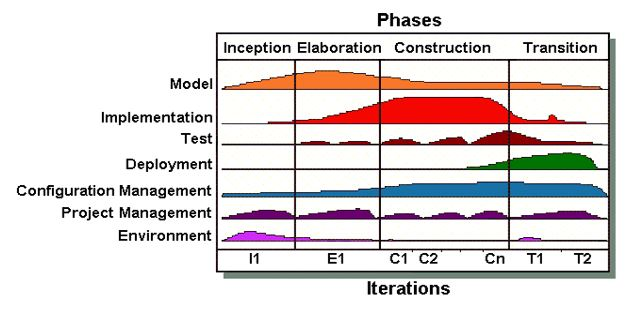
\includegraphics[width=15cm,height=9cm]{image/3-1.jpg}
	\caption{Rational Unified Process}
\end{figure}

\noindent\textbf{Phase 1:  Inception Phase}\\
\hspace*{1.5cm}The Inception phase is where the researchers get familiarity with the project goal and scope. It helps determine the project feasibility, what customer wants, and how the researchers will get into more resource consumable phase.
	
The researchers planned to integrate GetOldTweets in the system for the collection of data. To make sense of the collected data, topic modelling should be done. For the topic modelling, the researchers integrated Mallet. To analyze the data, visualization is needed. To visualize the generated topic models, the researchers planned to use GraphStream.
	

\noindent\textbf{Phase 2: Elaboration Phase}\\
\hspace*{1.5cm}This phase is one of the crucial parts in the development of the study since collecting the most significant requirements for the system takes place. In this phase, the researchers should be able to define and baseline the architecture of the system in order to provide a stable basis for the bulk of the design and implementation effort in the Construction Phase. 

This is where the researchers determine the requirements of the proposed system. This can be presented by the various modules/features based on your presented objectives.

\begin{figure}[H]
	\centering
	\caption{Flowchart}
	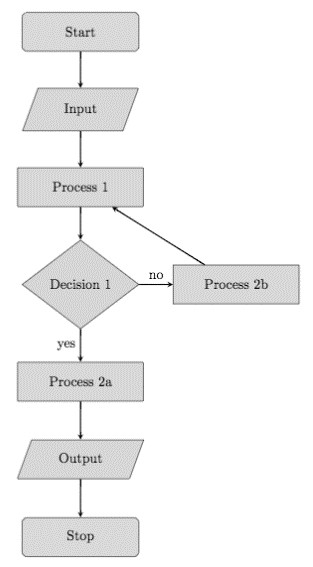
\includegraphics[width=7cm,height=11cm]{image/cs_flowchart.jpg}
\end{figure}


\noindent\textbf{Phase 3: Construction Phase}\\
\hspace*{1.5cm}The Construction Phase is about cost-efficient development of a complete product and operational version of the system that can be deployed in the user community. It is where the researchers develop a complete product that is ready for transition to its community. 
	
The researchers translated both the initial logical and physical designs to actual system development. The Java programming language was used by the researchers in the development of the system and tools were utilized to accomplish goals. The researchers used tools to accomplish our goals. For the data gathering, we used GetOldTweets1 an unofficial Java library for the Twitter 20 API and we used MAchine Learning for LanguagE Toolkit or MALLET2 for the topic modelling. MALLET is a Java-based package for statistical natural language processing, document classification, clustering, topic modelling, information extraction, and other machine learning applications to text. For the visualization, the researchers used GraphStream3, it is a tool for generating graphs, links and networks. We also used jFreeCharts for the visualization of the frequency of the words.

\subsection{Design of Software}
\vspace{-2ex}Software design is the process of transforming user requirements into appropriate abstracts which helps the researchers in designing, coding and implementing the developed software.

\begin{figure}[H]
	\centering
	\caption{Conceptual Framework}
	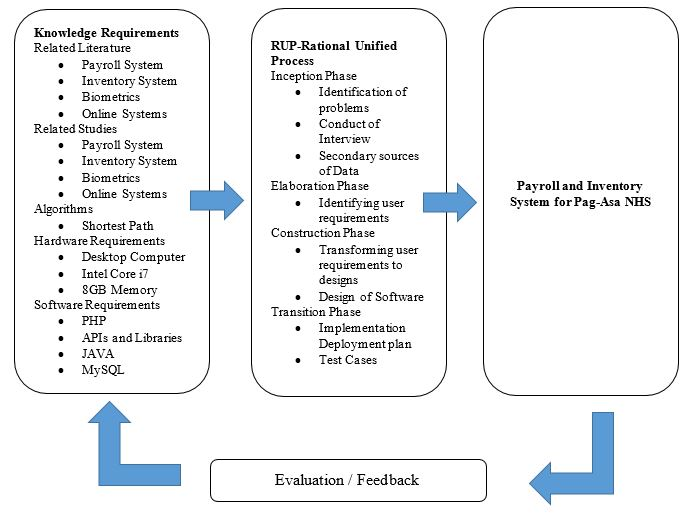
\includegraphics[width=15cm,height=11cm]{image/3-3.jpg}
\end{figure}
\noindent\textbf{Phase 4: Transition Phase}\\
\hspace*{1.5cm}The purpose of the transition phase is to transition the software product to the user community. In this phase the researchers validate the new system against user expectations. 
	
The researchers prepared test cases to ensure that the developed system requirements were met…

\begin{table}[H]
	\centering
	\caption{Software Requirements}
	\begin{tabular}{ | C{4cm} | C{6cm} | C{4cm} |} 
		\hline
		Component & Minimum	& Suggested \\
		\hline
		Browser & Google Chrome & Google Chrome \\
		\hline
		Apache, MySQL  and PHP	& Version 5 & Version 5.5 or latest \\
		\hline
		
	\end{tabular}
\end{table}

\begin{table}[H]
	\centering
	\caption{Hardware Requirements}
	\begin{tabular}{ | C{4cm} | C{6cm} | C{4cm} |} 
		\hline
		Component & Minimum	& Suggested \\
		\hline
		Disk Space & 10GB & 30GB \\
		\hline
		Memory Requirement & At least 512 MB of Random Access Memory (RAM) & 1GB of RAM \\
		\hline
		Processor &	Intel or AMD Processor, at least 1.06 GHz	& Intel or AMD Processor, 1.7 GHz \\
		\hline
	\end{tabular}
\end{table}

Every computer system has requirements in terms of Software and Hardware used for better implementation. In this case, the researchers listed in the table above the required software and hardware to be used in the proposed system.

%For your NLP process, you may include under the implementation phase of your methodology the following but not limited to: Data Collection, Data Filtering, Data Processing, Data Analysis. These NLP processes may also integrate discussion of the algorithm used, notations and formulas, evaluation methods, tools used, and other NLP concepts.\newpage
\clearpage
\thispagestyle{empty}
\addcontentsline{toc}{chapter}{\hspace{6mm}\textbf{CHAPTER 4 \hspace{8mm} RESULTS AND DISCUSSION \hspace{4.9cm}}}

\begin{center}
	\textbf{{CHAPTER 4}}\\
	\vspace{-1ex}
	\textbf{RESULTS AND DISCUSSION}
	\vspace{-3ex}
\end{center}

This chapter presents the results and analysis of findings made in the conduct of the study. (Objective #1) This includes discussion of the developed Topic Modelling Tool that can collect, pre-process and generates topic models. (Objective #2) The Latent Dirichlet Allocation algorithm used to generate topic models, and (Objective #3) the extent of correctness of the generated topic models based on its topic coherence.  

\subsection{Features of the Develop NLP Tool / Game / Application}
\vspace{-2ex}
{\textbf{Uploading of Data.}}  Data can be uploaded in the main interface window where the upload tab is located as shown in the figure below. The system accepts .txt data file as well as multiple .txt files placed in a folder. It follows mallet syntax for importing documents, import-dir command for multiple .txt files and import-file command for individual .txt file. \\
\vspace{-1ex}
	
    \begin{figure}[H]
            \centering
            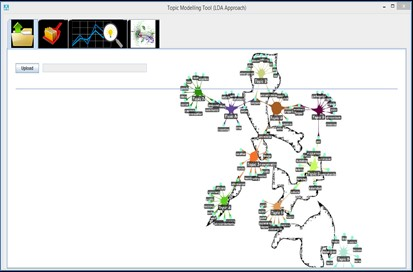
\includegraphics[width=15cm,height=9cm]{image/cs_figure1.jpg}
            \caption{Main Interface with the Upload Tab Window}
	\end{figure}
	
\textbf{Pre-processing of Data. }In the clean data tab shown in figure 2, the system included the default English Mallet stopwords to be deleted form the uploaded dataset. It allows user to view the default Mallet English stopwords, upload additional stopwords in .txt files, as well as create a new stoplist. Users can also add word or words that will automatically be added to the existing uploaded or created stoplists. 

Lastly, from the uploaded, created or added words in the list, users can also delete word or words by highlighting or selecting them. These cleaning options can assure that the topic model to be generated will be more appropriate.

    \begin{figure}[H]
	\centering
	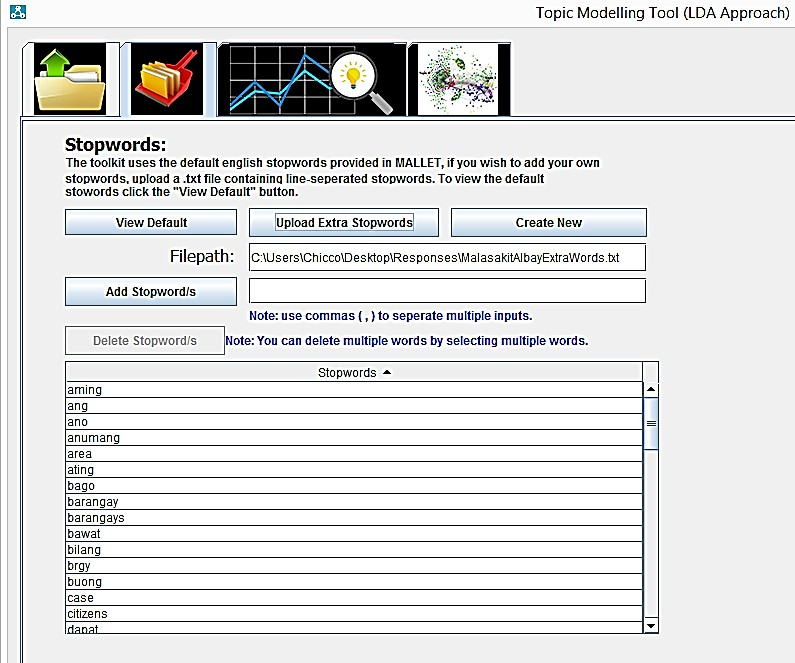
\includegraphics[width=13cm,height=7cm]{image/cs_figure2.jpg}
	\caption{Stopwords Options}
	\end{figure}

\textbf{Processing of Data.} Processing of the cleaned data sets starts with the click of the run button, the system then displays the required parameters in order for it to generate a topic model. The following parameters as shown in figure 3 are required to generate a topic model. Number of topic indicates the number of topic models the user wants to generate. Number of iterations normally starts from 50 to 500, up-to 10,000. Iteration depends on the size of the data sets.

The smaller the datasets, low iteration should be sensible. The number of words indicates the words per topic, optimization interval assigns the occurrence value based on the Latent Dirichlet Allocation (LDA), and the model name is the created file of the generated topic model. Clicking the start button will begin the processing to generate topic model with the given parameters. 

    \begin{figure}[H]
	\centering
	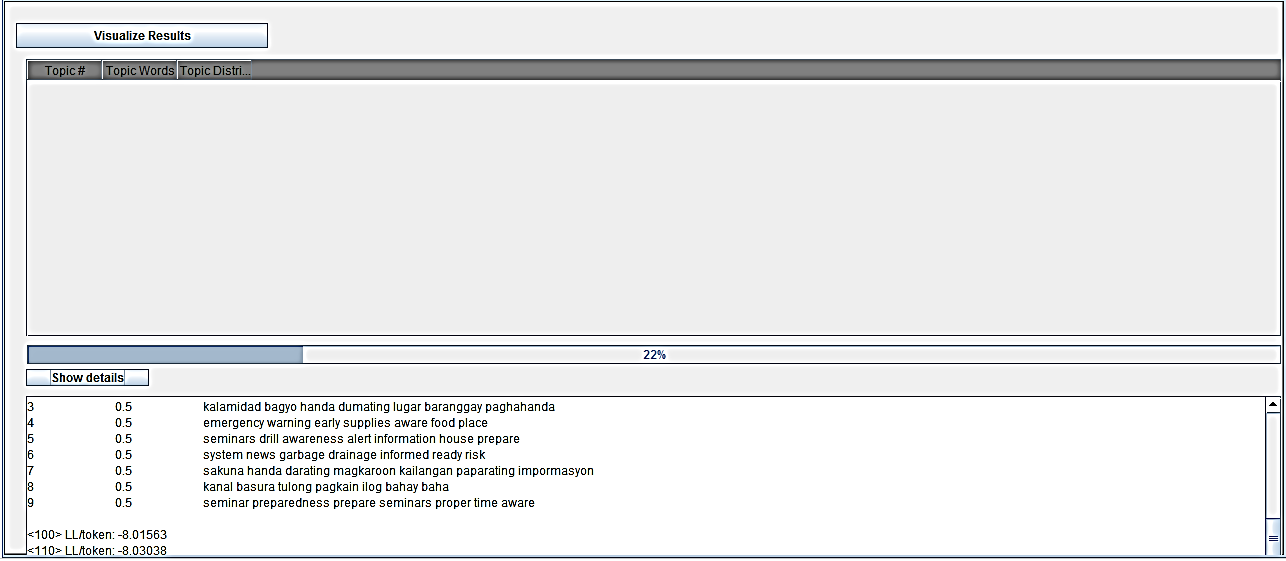
\includegraphics[width=13cm,height=7cm]{image/cs_figure3.png}
	\caption{Processing for Topic Modeling}
	\end{figure}

\textbf{Game Modes.} The Segregation Game is a 2D swipe-and-shoot game developed for android in order to teach the users how waste segregation is properly done. The game has two modes, the Player vs. A.I. mode in which the player will play against an A.I. opponent in easy, medium or hard difficulty, and the Player vs. Player mode in which the player will play against another player in a local area network or WLAN.

    \begin{figure}[H]
	\centering
	
\includegraphics[width=4cm,height=7cm]{image/cs_figure4_1.jpg}
	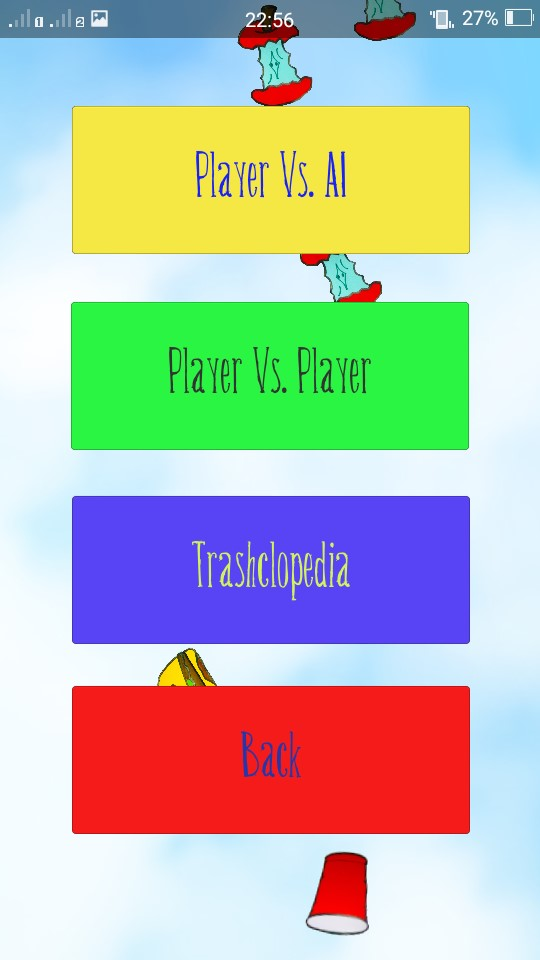
\includegraphics[width=4cm,height=7cm]{image/cs_figure4_2.jpg}
	\caption{The Segregation Game’s Main Menu and Game Modes}
	\end{figure}

\textbf{Difficulty Levels.} There are three difficulty levels in the game, the “easy” difficulty in which the opponent taps the screen in a slow pace (3 seconds), the “normal” difficulty in which the A.I. taps the screen in a faster pace (1.5 seconds) and the “hard” difficulty in which the A.I. taps the screen in the fastest pace (1 second).

\textbf{The “Trashclopedia”.} The “Trashclopedia” has three parts as seen in figure 5, the “Trash Talk”, the definition of terms regarding waste segregation, the “Trivia” has useful facts for the user’s knowledge and enjoyment, and the “Classification”, the classification of the in-game objects that are classified into biodegradable and non-biodegradable. 

    \begin{figure}[H]
	\centering
	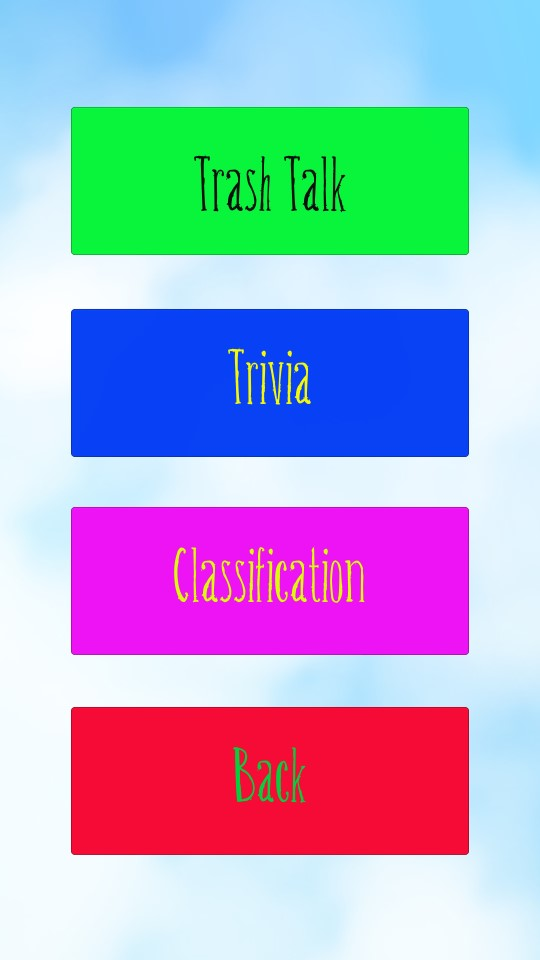
\includegraphics[width=4cm,height=7cm]{image/cs_figure5.jpg}
	\caption{The Trashclopedia}
	\end{figure}

\textbf{Latent Dirichlet Allocation (LDA) Algorithm used to appropriately categorize similar groups of data.}  In natural language processing, is a generative model that allows sets of observations to be explained by unobserved groups that explain why some parts of the data are similar. Using a plate notation to represent the Latent Dirichlet Allocation (LDA) approach, the dependencies among the many variables can be captured concisely. Figure 6 represents the following: The boxes are “plates” representing replicates; the outer plate represents documents, while the inner plate represents the repeated choice of topics and words within a document. M denotes the number of documents, N the number of words in a document.

    \begin{figure}[H]
	\centering
	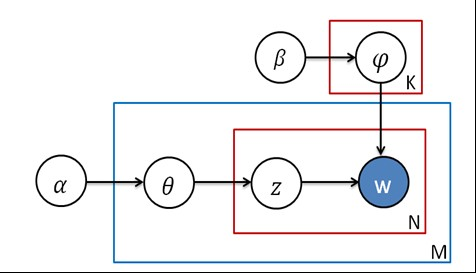
\includegraphics[width=12cm,height=7cm]{image/cs_figure6.jpg}
	\caption{Plate notation for LDA with Dirichlet-distributed topic-word}
	\end{figure}

\noindent Where:
\vspace{-2ex}
\begin{enumerate}
	\item [] α (alpha) is the parameter of the Dirichlet prior on the per-document topic distributions;
	\item [] β (beta) is the parameter of the Dirichlet prior on the per-topic word distribution;
	\item [] θ(theta)M  is the topic distribution for document M;
	\item [] φ(phi)K is the word distribution for topic K;
	\item [] Zmn is the topic for the n-th word in document M; and
	\item [] Wmn is the specific word.
\end{enumerate}

\subsection{Algorithm used for the Developed System / Application to achieve the necessary functions or output/s of the study.}

Latent Dirichlet Allocation (LDA) assumes documents are produced from a mixture of topics, these topics then generate words based on their probability distribution. Given a dataset of documents, LDA backtracks and tries to figure out what topics would create those documents. LDA is a matrix factorization technique. In vector space, any corpus can be represented as a document-term matrix.

\textbf{Parameters of Latent Dirichlet Allocaton (LDA).} Parameters are vital in the correctness of the generation of models in topic modeling. The following are the LDA parameters:

Alpha and Beta. Alpha and Beta hyper-parameters are the key parameters of LDA where alpha represents document-topic density and Beta represents topic-word density. Higher the value of alpha, documents are composed of more topics and lower the value of alpha, documents contain fewer topics. On the other hand, higher the beta, topics are composed of a large number of words in the corpus, and with the lower value of beta, they are composed of few words.

Number of Topics. These are the number of topics to be extracted from the corpus. Researchers have developed approaches to obtain an optimal number of topics by using Kullback Leibler Divergence Score.

Number of Topic Terms. The number of terms composed in a single topic where generally is determined according to the requirement. If the problem statement talks about extracting themes or concepts, it is recommended to choose a higher number, if problem statement talks about extracting features or terms, a low number is recommended.

Number of Iterations / passes. The maximum number of iterations allowed to LDA algorithm for convergence.
	
\textbf{Djikstra’s algorithm to compute the distances between nodes.} The Djikstra’s algorithm computes the distances between nodes as shown in figure 7. It gets the values of the designated paths and it computes the distances between the indexes which are represented as nodes in the map. The researchers plotted the nodes in each path through the x and y coordinates of the image. The nodes are called in the algorithm to determine the point of origin and the destination and to display the paths.

    \begin{figure}[H]
	\centering
	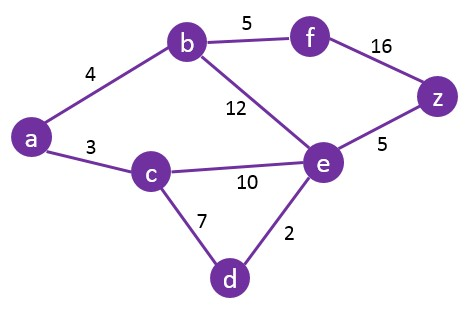
\includegraphics[width=12cm,height=7cm]{image/cs_figure7.jpg}
	\caption{Shortest Path using Djiktra Algorithm}
	\end{figure}

\textbf{Application of Recurrent Neural Network Algorithm in Disaster Management.} Recurrent neural network, shown in figure 8 is a type of ANN, where it takes input not just the current example they see, but also what they have perceived previously in time.  It has recurrent means of interpreting and assessing the current information being processed. RNN can utilize distributed representations of words by first converting the tokens comprising each text into vectors, which form a matrix. Networks main advantage resides in their ability to deal with sequential data. The prediction by the network at time-step T is influenced by the one it made at time-step T – 1.This chapter presents the results and analysis of findings made in the conduct of the study. (Objective #1) This includes discussion of the developed Topic Modelling Tool that can collect, pre-process and generates topic models. (Objective #2) The Latent Dirichlet Allocation algorithm used to generate topic models, and (Objective #3) the extent of correctness of the generated topic models based on its topic coherence.  

    \begin{figure}[H]
	\centering
	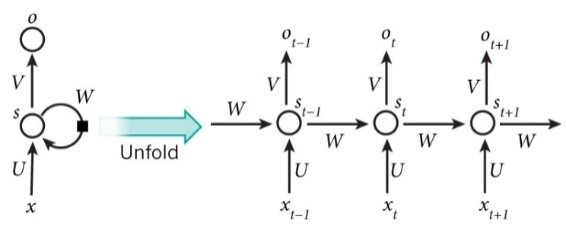
\includegraphics[width=12cm,height=6cm]{image/cs_figure8.jpg}
	\caption{Recurrent Neural Network}
	\end{figure}

%--------------------------------------------------------------------------------------------
\textbf{Extent of correctness of the generated topic models based on its topic coherence}

\textbf{Evaluating the Topic Models through Human Judgment.} The generated topic models can be measured by evaluating the performance of the Latent Dirichlet Allocation (LDA). Evaluating the LDA can be done using human judgments to examine the topics. This may involve identifying semantic coherent topics and measuring if topic model’s association agrees with human topic associations for a dataset. 

One method of measuring its correctness is by comparing the directly annotated topic assignments based on its top-N words and validate if these annotations agree with the human judgment. 

\textbf{Model Precision.} Model precision was used to measure the correctness of the generated topic model against manually annotated models. It is the number of agreements between humans and the model divided by the total number of judgments. Table 1 presents the results to measure the correctness of the generated topic model against the manually annotated ones. Test 1 returned 100\% precision, test 2 with 83\% precision and test 3 returned an 85\% precision. 
In summary, the average precision rated 87\% denoting that the manual annotations of the generated topic models agreed with the human judgments. The respondents view on the topics marked with “No Label” disagreed to their judgment implying that there could be themes assigned. These were true enough because finding shows that the topics have coherent aspects but words were evenly distributed indicating possible assignments of multiple labels.



\begin{table}[H]
	\centering
	\caption{Precision Results}
	\centering
	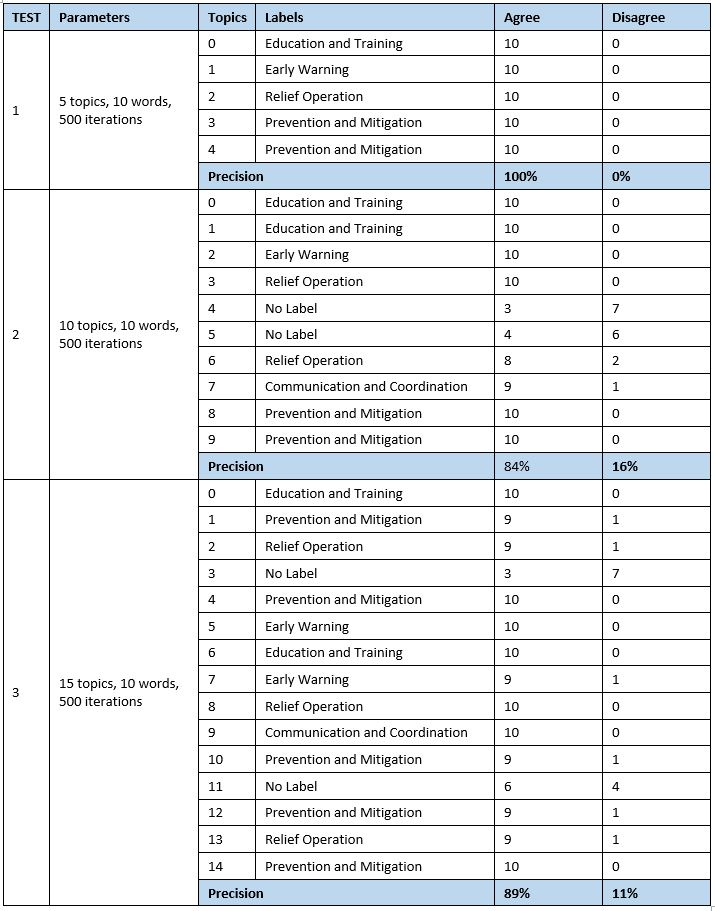
\includegraphics[width=12cm,height=16cm]{image/cs_table1.jpg}
\end{table}

\subsection{Performance Evaluation of the Classification Models using accuracy, precision F measures and recall metrics. }

\textbf{Performance Evaluation.} Performance of the classification models were described by the confusion matrices which were used to properly present the classified data. The classifier configuration that obtained the best accuracy was selected to be used in developing the DRM e-Participatory toolkit qualitative response classification system. The average accuracy, precision, recall were computed to give overall assessment of the effectiveness of the classification across the defined categories for the DRM qualitative responses.

Accuracy measured the effectiveness of the classifier in terms of detections in agreement with the actual classifications.  Formula 1 shows the formula on determining the accuracy of the model.

%Formula 1
\begin{center}
Formula 1. \textit{ Accuracy}
\end{center}
\vspace{-2ex}
\begin{equation}
\begin{align*}
Accuracy &= \frac{No. of Correctly Classified Responses}{Total no.of Qualitative Responses}\
\end{align*}
\end{equation}
%Formula 1

On the other hand, precision measured the exactness of a classifier and considers false detection. A higher precision means less false positives, while a lower precision means more false positives. Formula 2 shows how precision is computed.

%Formula 2
\begin{center}
Formula 2. \textit{Precision}
\end{center}
\begin{equation}
\begin{align*}
Precision &= \frac{True Positives}{True positives + False positives}\
\end{align*}
\end{equation}

%Formula 2

Recall measures the completeness, or sensitivity, of the classifier. Higher recall means less false negatives, while lower recall means more false negatives.

%Formula 3
\begin{center}
Formula 3. \textit{Recall}
\end{center}
\begin{equation}
\begin{align*}
Recall &= \frac{True Positives}{True positives+False negatives}\
\end{align*}
\end{equation}
%Formula 3


The last metric, which is F-measure is computed using the formula shown below. It is the weighted harmonic mean of precision and recall and its main advantage is it is able to rate a system with one unique rating. 

%Formula 4
\begin{center}
Formula 4. \textit{F-measure}
\end{center}
\begin{equation}
\begin{align*}
F - measure &= \frac{2*precision*recall}{precision + recall}\
\end{align*}
\end{equation}
%Formula 3

\textbf{Results of Experiments.} The performance of the classification models were determined by the standard metrics discussed in the previous section. Metric scores of regular and bidirectional neural networks are shown in table 2. It is observed that the two RNN algorithms produced closed evaluation results where Bidirectional RNN obtained accuracy rate of  81.67\%, 81.17 precision, 81.67\% recall and 80.81\% f-measure against performance evaluation result of regular RNN where is obtained 81.25\% accuracy, 80.84\% precision, 81.25\% recall and 80.25\% f-measure.

\begin{table}[H]
	\centering
	\caption{Summary of Precision Results}
	\begin{tabular}{ | C{3cm}| C{3cm} | C{3.5cm} |}
	\hline
	\textbf{Standard Metric} & \textbf{Regular RNN} & \textbf{Bidirectional RNN}\\
	\hline 
	\textbf{Accuracy} & 81.25\% & \textbf{81.67\%}\\
	\hline
	\textbf{Precision} & 80.84\% & \textbf{81.17\%}\\
	\hline
	\textbf{Recall} & 81.25\% & \textbf{81.67\%}\\
	\hline
	\textbf{F-measure} & 80.25\% & \textbf{80.81\%}\\
	\hline
	\end{tabular}
\end{table}


\newpage
\clearpage
\thispagestyle{empty}

\addcontentsline{toc}{chapter}{\hspace{6mm} \textbf {CHAPTER 5} \hspace{7mm} \textbf {SUMMARY, FINDINGS, CONCLUSIONS AND \\ \hspace*{3.9cm}  RECOMMENDATIONS} \hspace{6.3cm}}

\begin{center}
	\textbf{{CHAPTER 5}}\\
	\vspace{-1ex}
	\textbf{SUMMARY, FINDINGS, CONCLUSIONS AND RECOMMENDATIONS}
	\vspace{-2ex}
\end{center}

This chapter presents the Summary of Findings, Conclusions, and Recommendations of the study Topic Modelling on Mayon Volcano Tweets using Latent Dirichlet Allocation (LDA).

\subsection{Summary of Findings and Accomplishments}
\vspace{-2ex}Based on the objectives of the study, the following results were accomplished:

\vspace{-2ex}
\begin{enumerate}
	\item {\textbf{\textcolor{red}{The Develop Tool/Application/System.} Sample 1.} Integrating game elements in the developed 2 dimensional Digital Netiquette Gamification for android was able to capture users’ interests and increase their awareness about sensitive issues such as digital netiquette.\\
	\textbf{Sample 2. }The developed topic modeling tool was able to collect, pre-process, generate topic models as well as visualize these models that provided the unique meaning of the collected dataset.\\
	\textbf{Sample 3.} Utilizing online open-source dataset using getold tweets was able to produce enough data to generate appropriate models. A total of 38,888 tweets consisting of specified keywords and date were successfully collected.
	
	\item \textbf{\textcolor{red}{The algorithm used for the Developed System / Application to achieve the necessary functions or output/s of the study.} Sample 1.} Utilizing the Iterative Dichotomiser 3 (ID3) Algorithm through the incorporation of a decision tree and reward system was able to evaluate users’ learning progress.\\
	\textbf{Sample 2.} The Latent Dirichlet Allocation Algorithm was able to generate topic models by appropriately categorizing similar groups of data in a datasets to determine similar topics from the collected disaster-related responses.\\
	\textbf{Sample 3.} The Standard and Bidirectional Recurrent Neural Network was effective in terms of classifying typhoon related corpus and was able to generate relevant models.
	
	\item \textbf{\textcolor{red}{Assessing the users’ knowledge through pre and post evaluation test / Extent of correctness of the generated topic models based on its topic coherence / Performance Evaluation of the Classification Models using accuracy, precision F measures and recall metrics.}}\\
	\textbf{Sample 1.} The pre-evaluation and post-evaluation test was able to assess the users’ knowledge learned as applied in the real-situational scenarios before and after using the gamification.\\
	\textbf{	Sample 2.} Manual evaluation through human judgment was used to manually evaluate topic models by ranking topic significance as well as topic to words similarity. This provided a more inclusive result of the true quality of the different topic models.\\
	\textbf{Sample 3.} The performance of the classification models were determined by the standard metrics. It was observed that the two RNN algorithms produced closed evaluation results where Bidirectional RNN obtained accuracy rate of  81.67\%, 81.17 precision, 81.67\% recall and 80.81\% f-measure against performance evaluation result of regular RNN where is obtained 81.25\% accuracy, 80.84\% precision, 81.25\% recall and 80.25\% f-measure.
\end{enumerate}
\vspace{-2ex}

\subsection{ Conclusions}
\vspace{-2ex}Based from the findings, the researchers came up with the following conclusions:
\vspace{-2ex}
\begin{enumerate}
	\item \textbf{Sample 1} Integrating game elements such as trophies, badges, power ups, sounds and animation in the developed gamification increased the interests of users to use the application. \\
	\textbf{Sample 2.} The features of the proposed system can easily upload datasets to be cleaned, analyzed, processed in-order to generate appropriate topic models as well as visually present the topic models to better present and appreciate the generated results.\\
	\textbf{Sample 3.} Integrating the collection, pre-processing, generation of models, visualizing as well as evaluating the models in the developed tool provided an easier methods of Classifying datasets.
	
	\item \textbf{Sample 1.} Using a Decision Tree which utilizes the Iterative Dichotomiser 3 (ID3) Algorithm provided a real scenario based decision making application that measures users’ progress based on the provided storyline. \\
	\textbf{Sample 2.} The Latent Dirichlet Allocation (LDA) algorithm was able to generate topic models by appropriately categorizing similar groups of data in a datasets to determine similar topics from the collected disaster-related responses.\\
	\textbf{Sample 3.} The process of classification of Typhoon Yolanda related tweets with relatively high accuracy was made possible using the sequential process of standard and bidirectional Recurrent Neural Networks (RNN) and their powerful architecture which remembers the past and future context of data.
	
	\item \textbf{Sample 1.} The pre-evaluation and post-evaluation tests was able to determine whether the user gained knowledge in proper computer etiquette before and after using the application.\\
	\textbf{Sample 2.} The use of both standard and bidirectional recurrent neural network algorithms in sentiment analysis were effective since it was able to achieve scores higher than 80\% in all evaluation metrics.\\
	\textbf{Sample 3.} The result of the evaluation on the extent of correctness of the generated topic models based on the top-N words using model precision yielded 87\% mean denoting that the manual annotations of the generated topic models agreed with the human judgments.
	
\end{enumerate}

\noindent
\subsection{ Recommendations}
\vspace{-2ex}On the basis of the conclusions, the researchers come up with several recommendations.  
\vspace{-3ex}
\begin{enumerate}
	\item Other features, modules of the develop system / application / tool / datasets
	\item Include other possible algorithms, comparison of algorithms, other methods
	\item Other test metrics, higher / better models, better results
\end{enumerate}\newpage
\clearpage
    \vspace*{\fill}
        \begin{center}
            \begin{minipage}{.6\textwidth}
                
                    \section{BIBLIOGRAPHY}
                
            \end{minipage}
        \end{center}
    \vfill
\clearpage

\newpage
%-----------Start book format--------------
%\begin{center} \textbf{A. BOOKS}\end{center}
%\vspace{2pt}
\begin{singlespace}
	\hangindent=\parindent
	\hangafter=1
	
	Blei, David M.et. al., Latent Dirichlet allocation. Journal of Machine Learning Research. 3: 993–1022. doi:10.1162/jmlr.2003.3.4-5.993, January 2003.\par
	Nouali, N., Bendjoudi, A., Bouchama, N., Guellati, N. Information Technology for Enhancing Disaster Management. Conference: Congrès National des Télécommunications et leurs Applications, At University of Béjaia, Algeria, May 2009\par
	Brynjar Gretarsson, et. al., TopicNets: Visual Analysis of Large Text Corpora with Topic Modeling ACM Transactions on Intelligent Systems and Technology (TIST) Volume 3 Issue 2, ACM New York, NY, USA, 2012. (more than 5 authors)\par
	Ligutum, C. et., al. Using Topic Modelling to make Sense of Typhoon-Related Tweets. 2016 International Conference on Asian Language Processing (IALP). Tainan, Taiwan, November 2016.\par
	P. Anupriya and S. Karpagavalli, LDA based topic modeling of journal abstracts. 2015 International Conference on Advanced Computing and Communication Systems, Coimbatore, 2015, pp. 1-5.\par
	Ostrowski, David Alfred, Using latent dirichlet allocation for topic modelling in twitter. 2015 IEEE International Conference on Semantic Computing, March 2015.\par
	
\end{singlespace}
%----------- End Magazine and Newspaper Articles format--------------

%-----------Start Website or Webpage format--------------

%----------- EndWebsite or Webpage format format--------------\newpage


\clearpage
\thispagestyle{empty}
    \vspace*{\fill}
        \begin{center}
            \begin{minipage}{.5\textwidth}
                
                    \section{APPENDICES}
             
            \end{minipage}
        \end{center}
    \vfill
\clearpage

\newpage
% Start Appointment of Capstone Project 2 Evaluators

\begin{center} 
	\textbf{\myappendix{Letters and Appointment}}
	
\includegraphics[width=14cm,height=18cm]{image/a1.JPG}
\end{center}

% End Appointment of Capstone Project 2 Evaluators
\newpage

%Start Appointment of Capstone Project 2 Evaluators #1


\begin{center} 
	
\includegraphics[width=14cm,height=18cm]{image/a2.JPG}
\end{center}
%End Appointment of Capstone Project 2 Evaluator #1

\newpage

% Start Appointment of Capstone Project 2 Evaluator #2


\begin{center} 
	
\includegraphics[width=14cm,height=18cm]{image/a3.JPG}
\end{center}

% End Appointment of Capstone Project 2 Evaluator #2 

\newpage

% Start Appointment of Capstone Project 2 Evaluator #3


\begin{center} 
	
\includegraphics[width=14cm,height=18cm]{image/a4.JPG}
\end{center}

% End Appointment of Capstone Project 2 Evaluator #3


\newpage
%Start Appointment Letter for Programming Adviser


\begin{center} 
	
\includegraphics[width=14cm,height=18cm]{image/a5.JPG}
\end{center}

%Start Appointment Letter for Content Adviser
\newpage
\begin{center} 
	
\includegraphics[width=14cm,height=18cm]{image/a6.JPG}
\end{center}


%End Appointment Letter for Content Adviser
\newpage
\begin{center} 
    \textbf{\myappendix{Interview Questionnaires}}
	
\includegraphics[width=14cm,height=15cm]{image/appendix_b.PNG}
\end{center}
\newpage
\begin{center} 
    \textbf{\myappendix{Software Project Management Plan}}
\end{center}

    \begin{center}
    \textbf{Gantt Chart/PERT}
    \end{center}
    
\begin{center}
 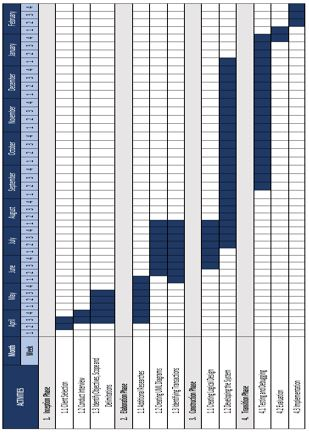
\includegraphics[width=15cm, height=18cm]{image/c1.jpg}
\end{center}

\newpage
    \begin{center}
    \textbf{\myappendix{Individual Tasking Table}}
	\end{center}

    \begin{center}
    	\setstretch{1}
    	\begin{tabular}{ | L{.5cm}| C{3cm} | C{6cm} | C{3cm} |} 
    		\hline
    		& Activity & Description & Person Responsible \\
    		\hline
    		1  & Data Gathering  & Interview with the CSC IT Dept. head   & All Members \\
    		\hline
    		2  & Chapter 1 of Research Paper  & Introduction, Objectives, Scope and Delimitations  & Ciara Peñarubia \\
    		\hline
    		3  & Chapter 2 of Research Paper & Related Literature and Studies  & Ciara Peñarubia \\
    		\hline
    		4  & 2nd Data Gathering  & For sample forms and additional information & All members \\
    		\hline
    		5  & Database Design & Database design & Klarenz Monreal \\
    		\hline
    		6  & User Stories   & Create user stories/ requirements  & Jasper Jules Balbuena \\
    		\hline
    		7  & Chapter 3 of Research Paper & Research Design and Methodology & Jasper Jules Balbuena \\
    		\hline
    		8  & Diagrams   & Including Use Case and DFD  & All Members \\
    		\hline
    		9  & Revise Chapter 2 &   Revise chapter 2  &  Ciara Peñarubia \\
    		\hline
    	\end{tabular}
	\end{center}	
	

\newpage

\begin{center} 
 \textbf{\myappendix{Diagrams} }
 \textbf{Entity Relationship Diagram}
\end{center}
\begin{center}
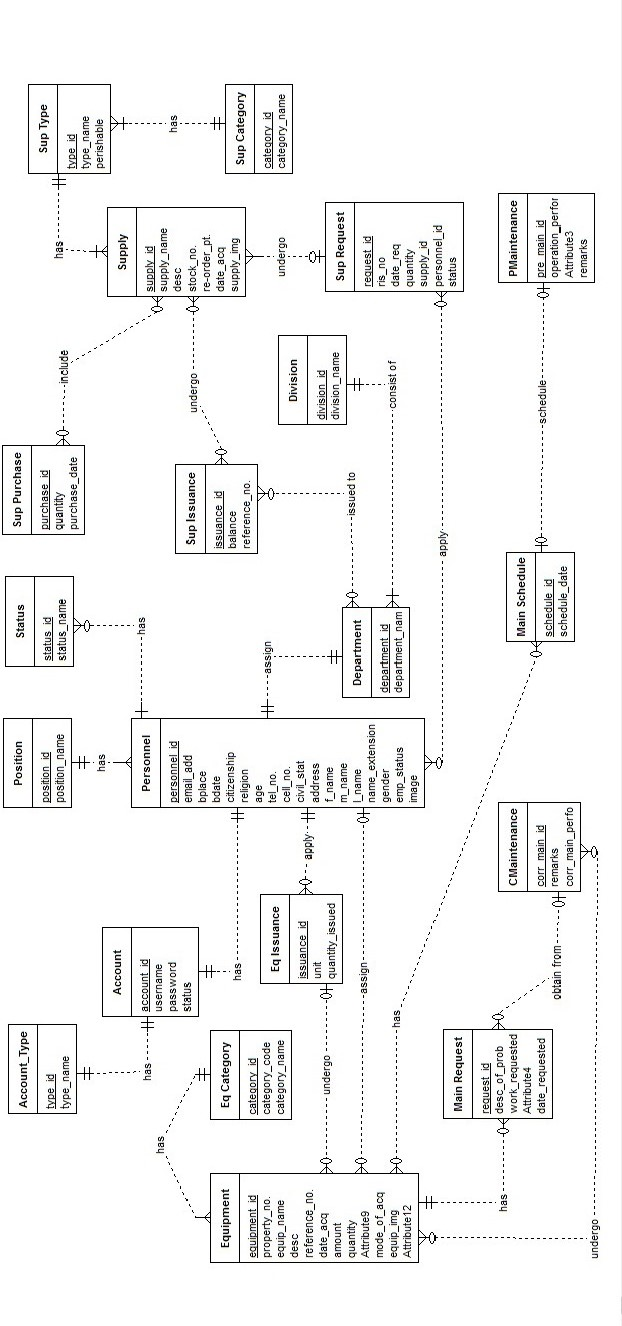
\includegraphics[width=14cm,height=18cm]{image/E.jpg}
\end{center}
\vfill

\newpage

\begin{center} 
	\textbf{Class Diagram}
\end{center}
\begin{center}
	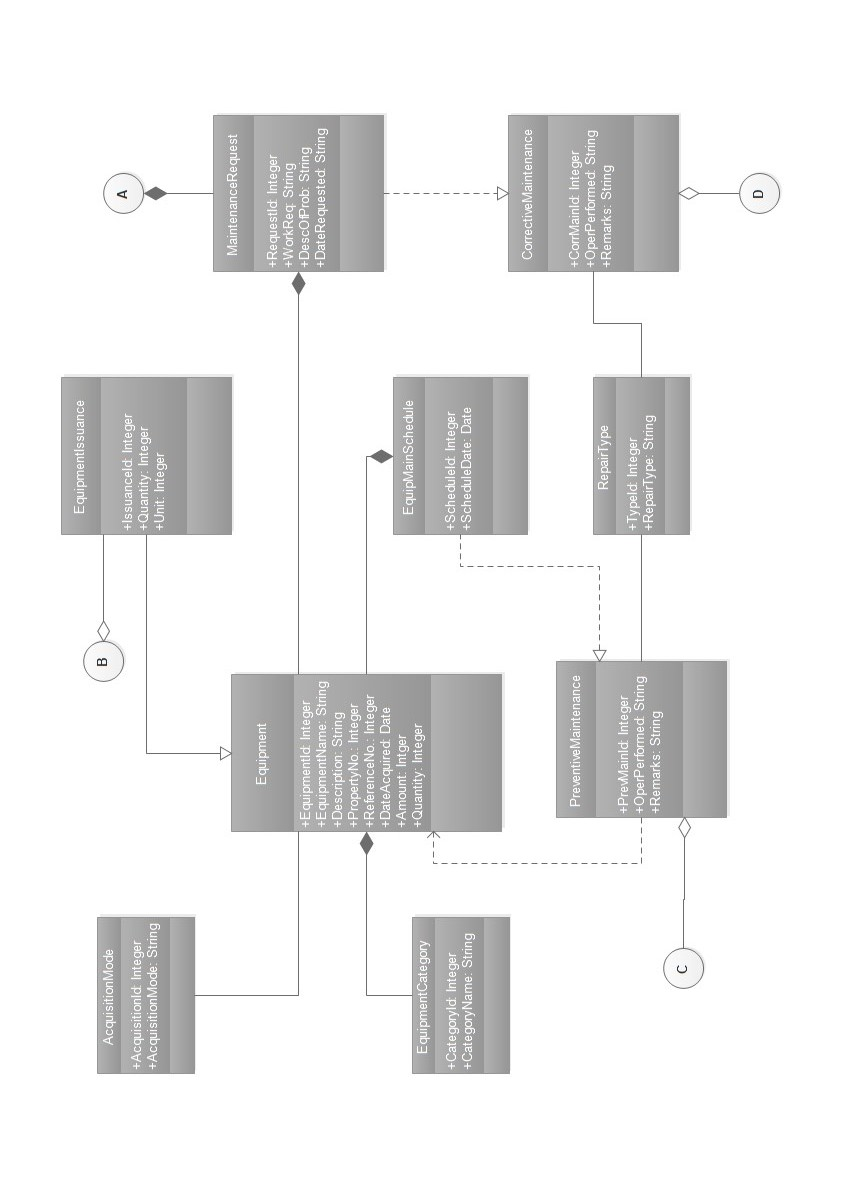
\includegraphics[width=14cm,height=18cm]{image/f1.jpg}
	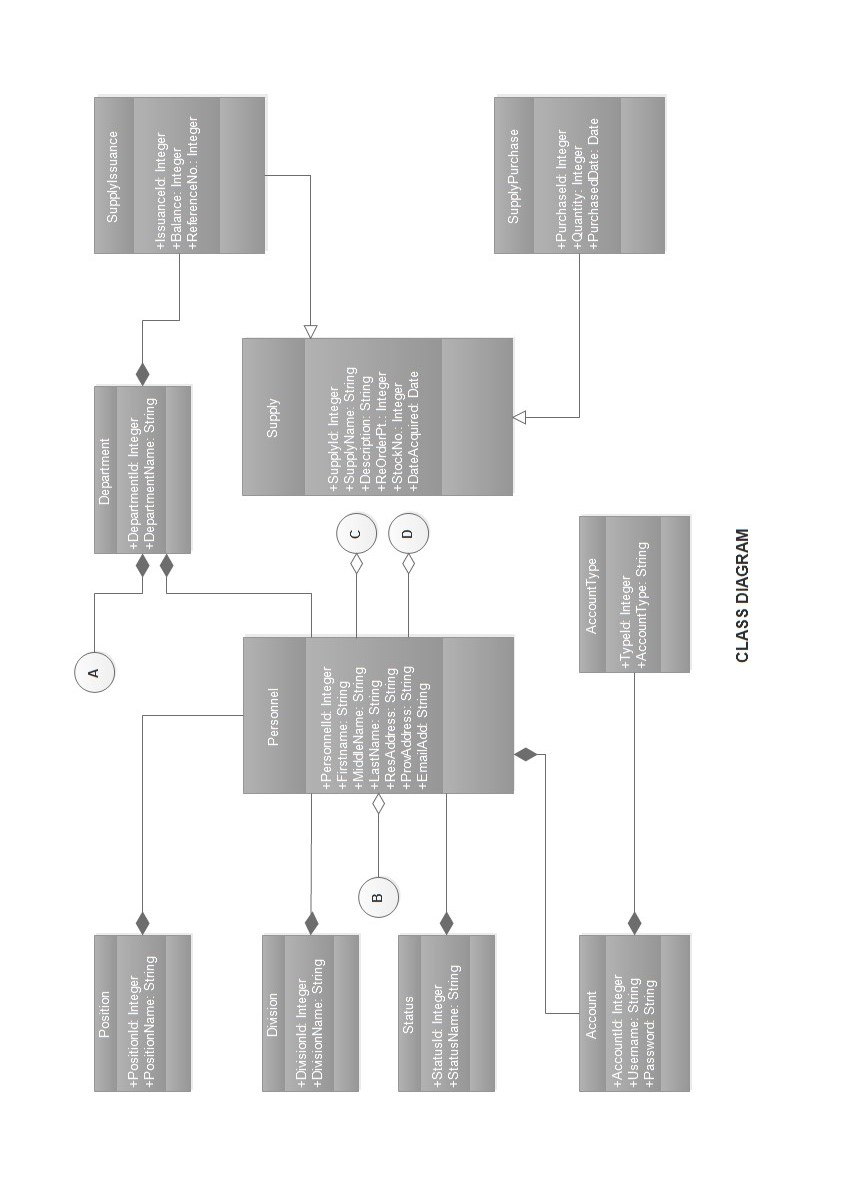
\includegraphics[width=14cm,height=18cm]{image/f2.jpg}
\end{center}
\vfill

\newpage

\begin{center} 
	\textbf{Use Case Diagram}
\end{center}
\begin{center}
	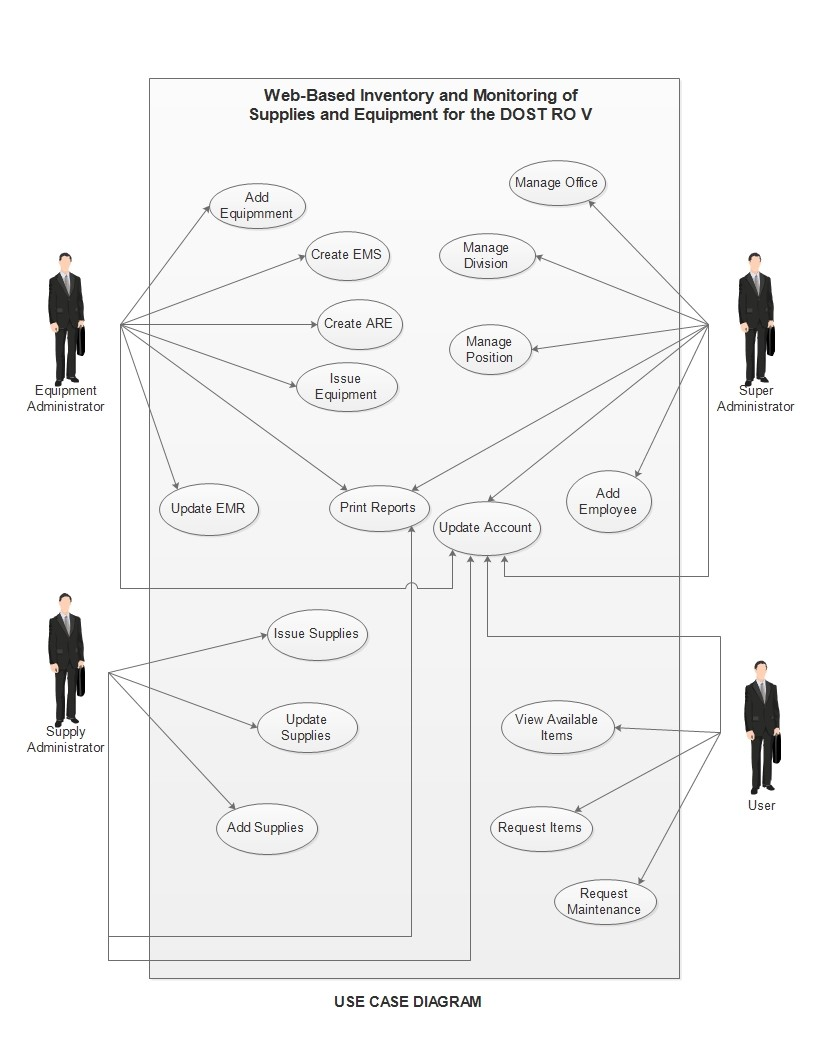
\includegraphics[width=14cm,height=18cm]{image/d-1.jpg}
\end{center}
\vfill

\newpage

\begin{center} 
	\textbf{Activity Diagram}
\end{center}
\begin{center}
	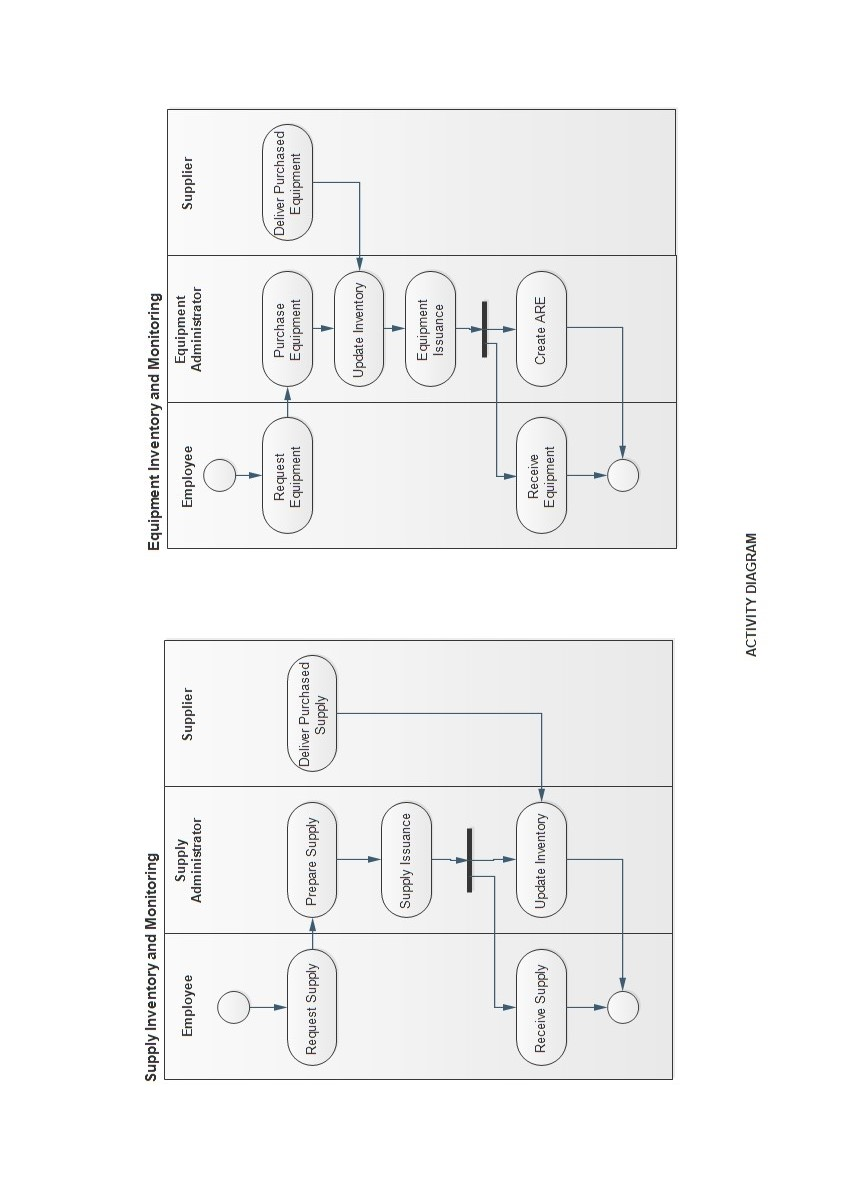
\includegraphics[width=14cm,height=18cm]{image/g1.jpg}
	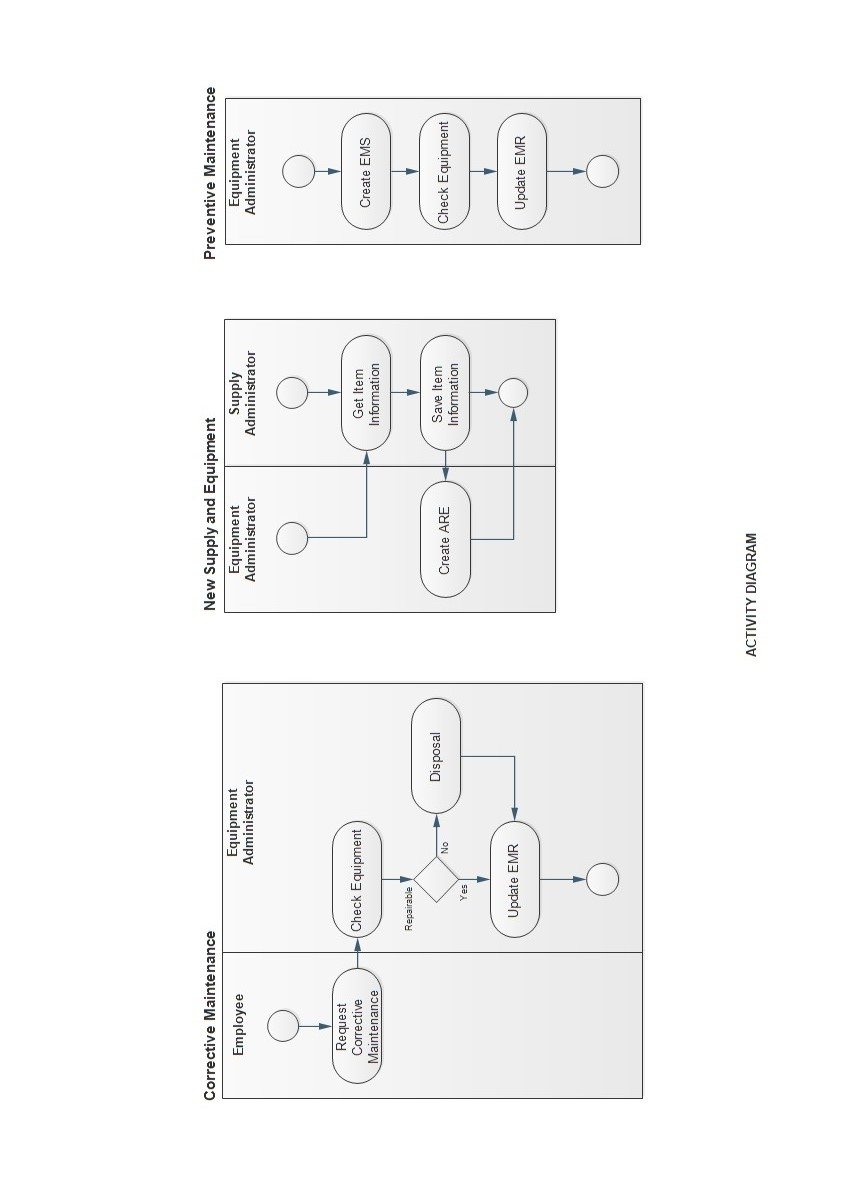
\includegraphics[width=14cm,height=18cm]{image/g2.jpg}
\end{center}
\vfill



\newpage
\begin{center} 
	\textbf{User Interface Design}
\end{center}
\begin{center}
	\textbf{User Interface Design \\}
	\vspace{5pt}
	
\begin{flushleft}
	\textbf{User}
\end{flushleft}

\begin{center}
	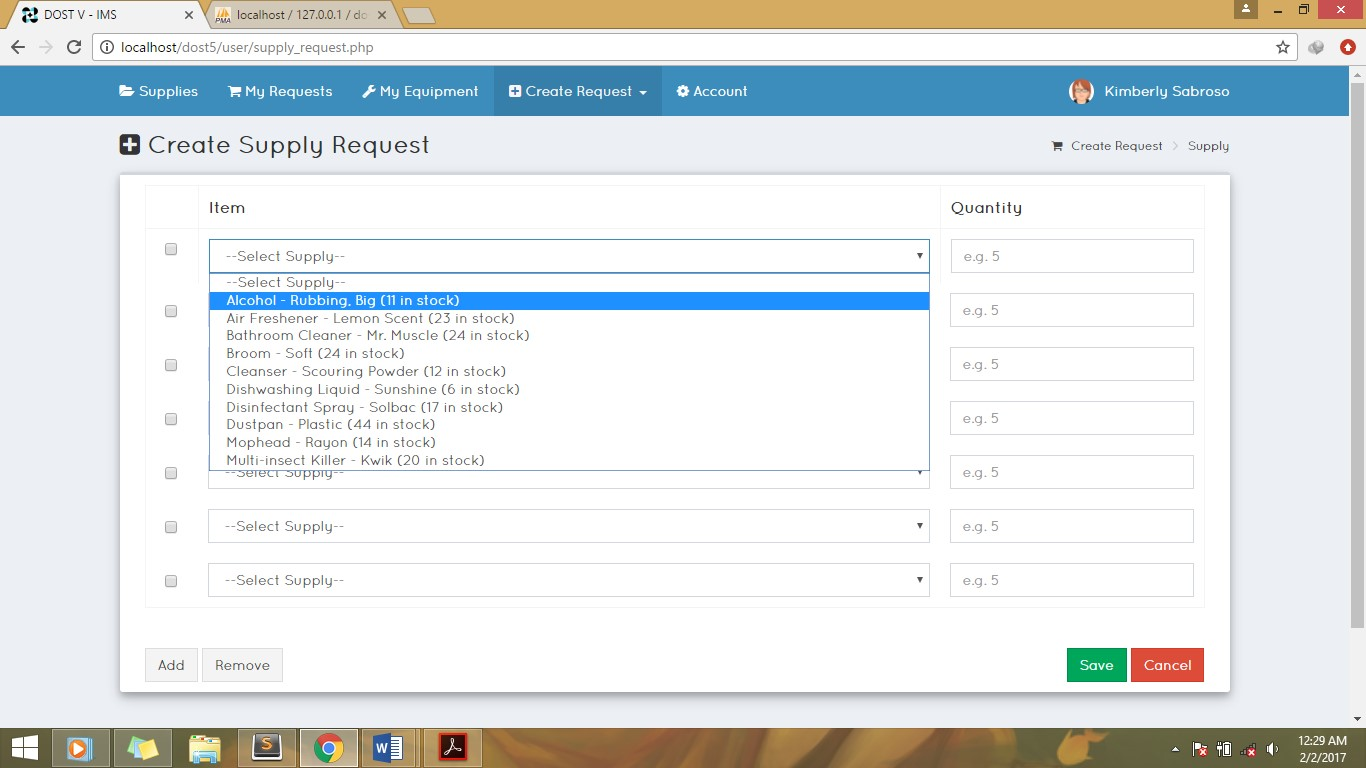
\includegraphics[width=13cm,height=8cm]{image/d3-1.jpg}\\
	Creating Request for Supply \\
	\vspace{1.5cm}
	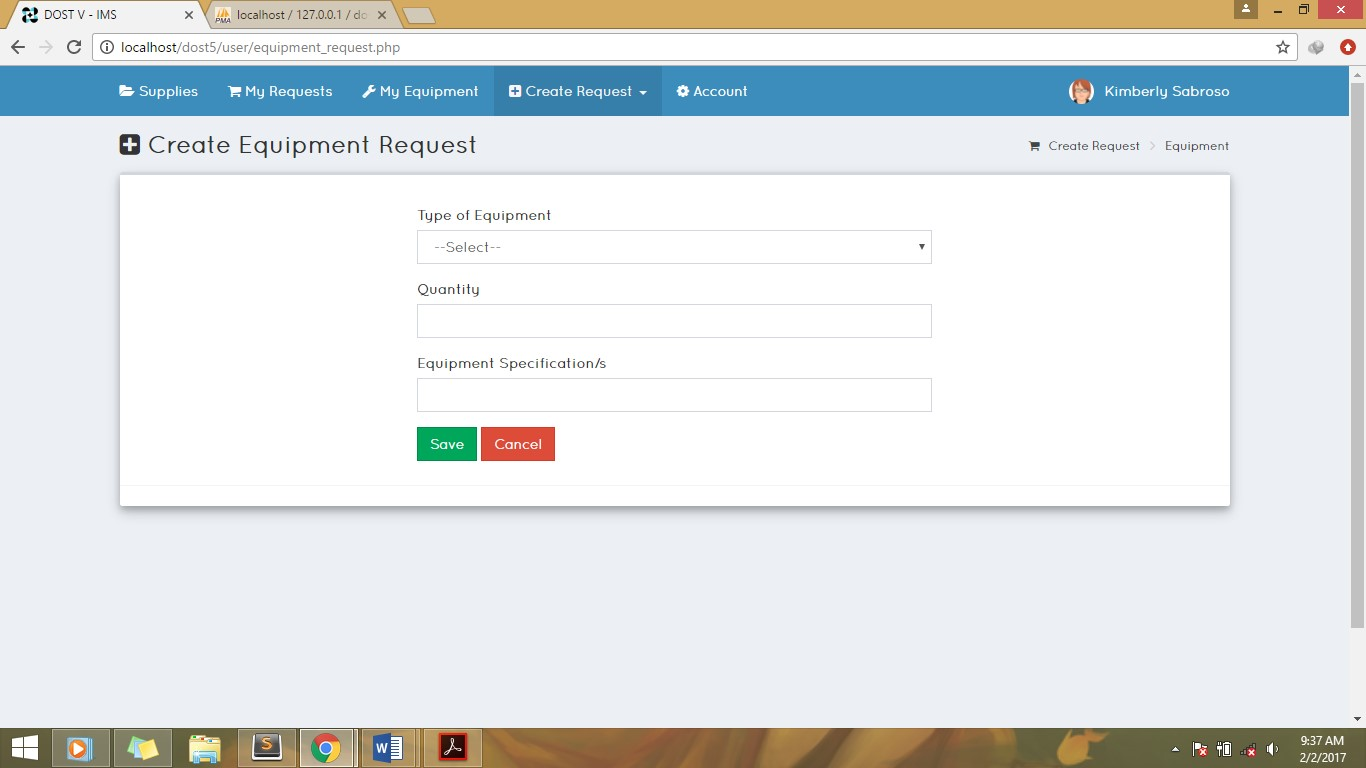
\includegraphics[width=13cm,height=8cm]{image/d3-2.jpg}\\
	Creating Request for Equipment \\
	\vspace{1.5cm}
	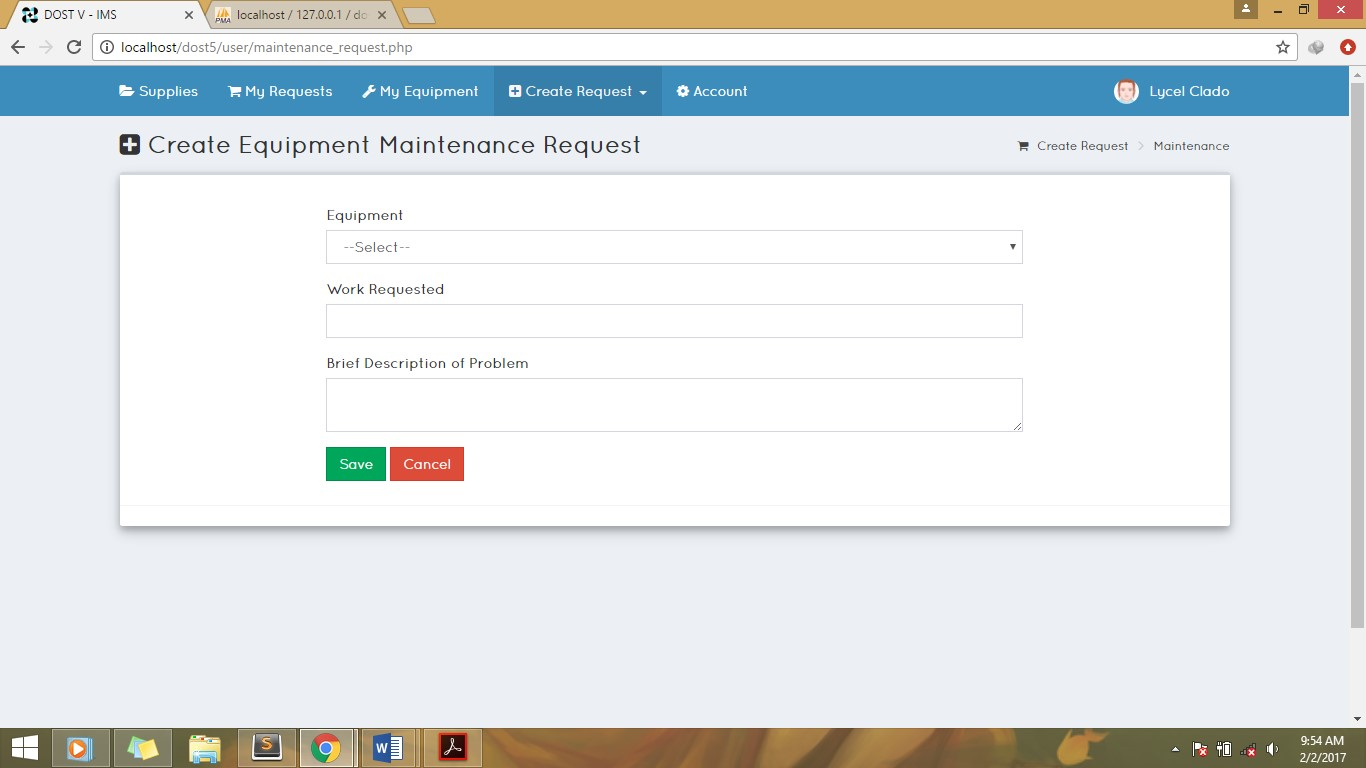
\includegraphics[width=13cm,height=8cm]{image/d3-3.jpg}\\
	Creating Request for Maintenance\\
	\vspace{1.5cm}
	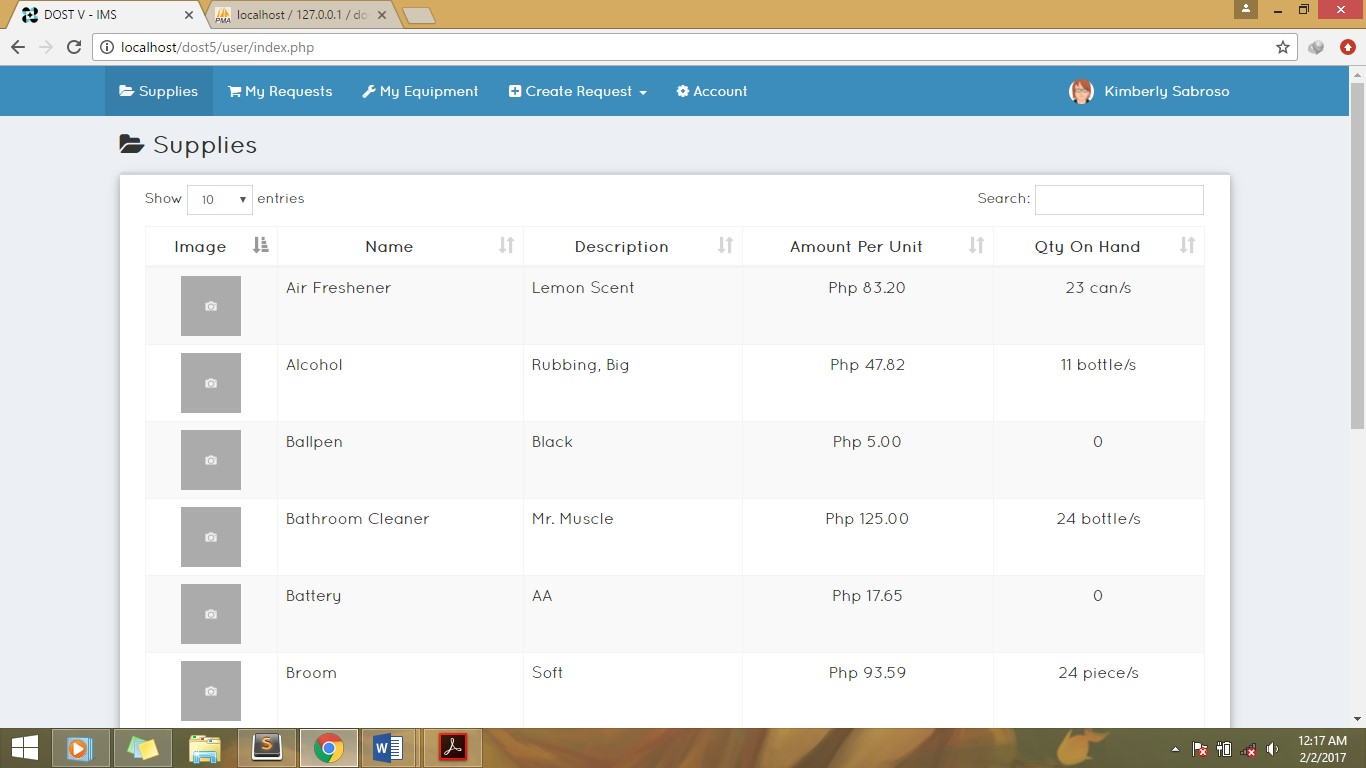
\includegraphics[width=13cm,height=8cm]{image/d3-4.jpg}\\
	List of Supplies\\
	\vspace{1.5cm}
	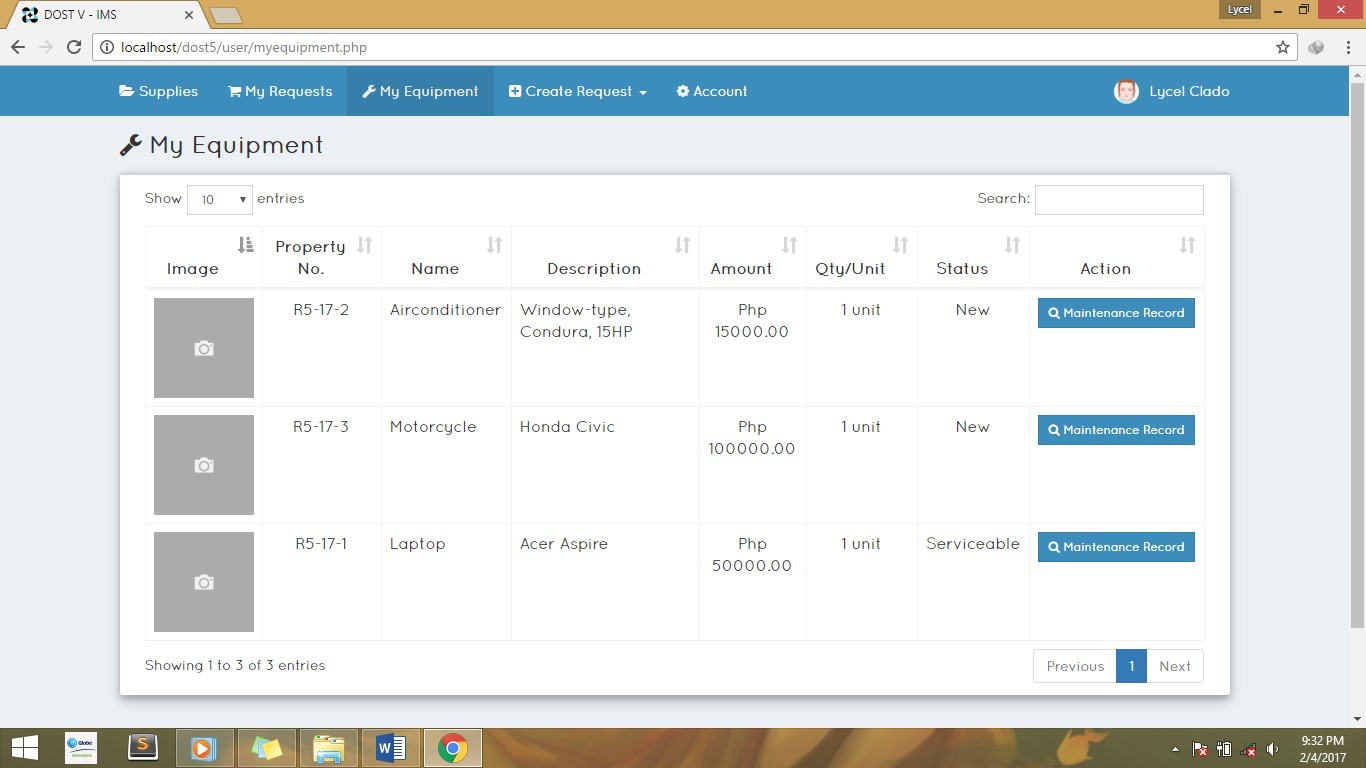
\includegraphics[width=13cm,height=8cm]{image/d3-5.jpg}\\
	List of Assigned Supplies\\
\end{center}


\begin{flushleft}
	\textbf{Supply Administrator}
\end{flushleft}	

\begin{center}
	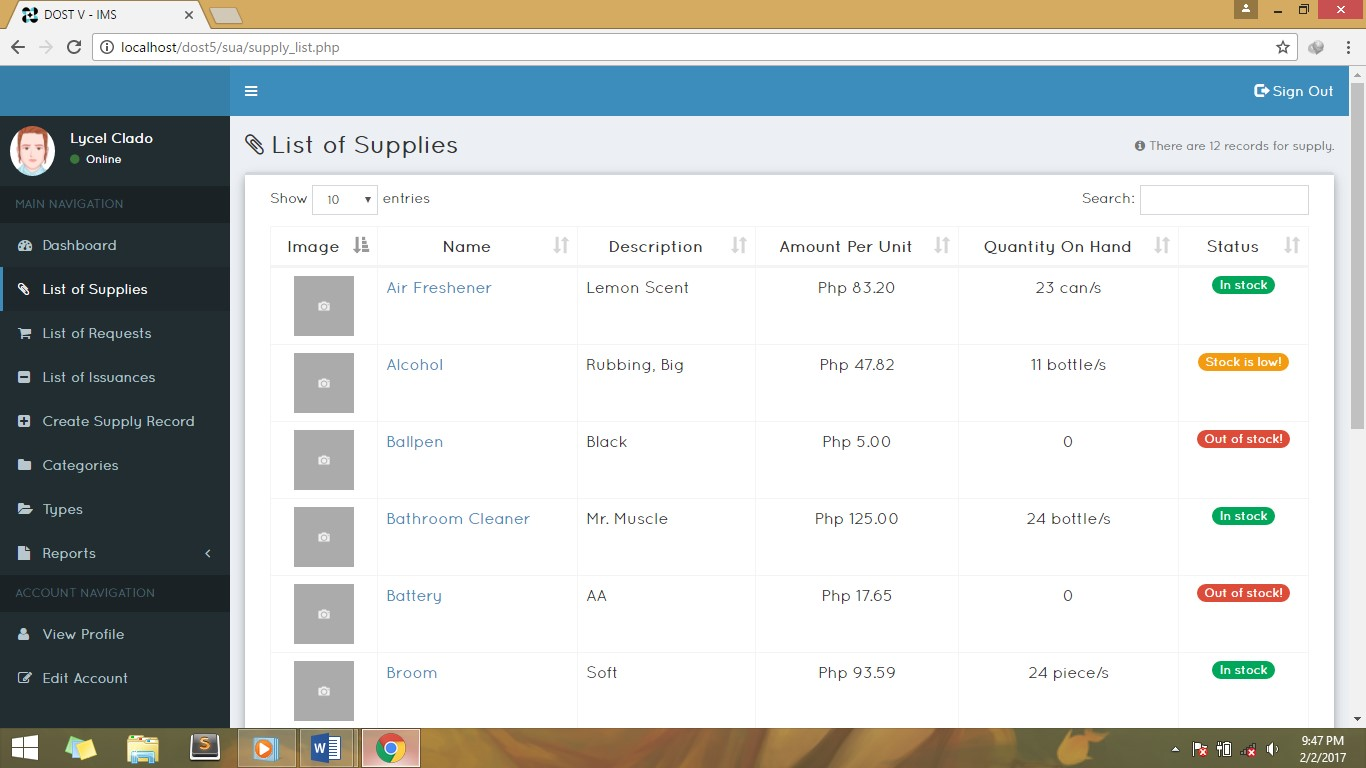
\includegraphics[width=13cm,height=8cm]{image/d3-6.jpg}\\
	List of Supplies \\
	\vspace{1.5cm}
	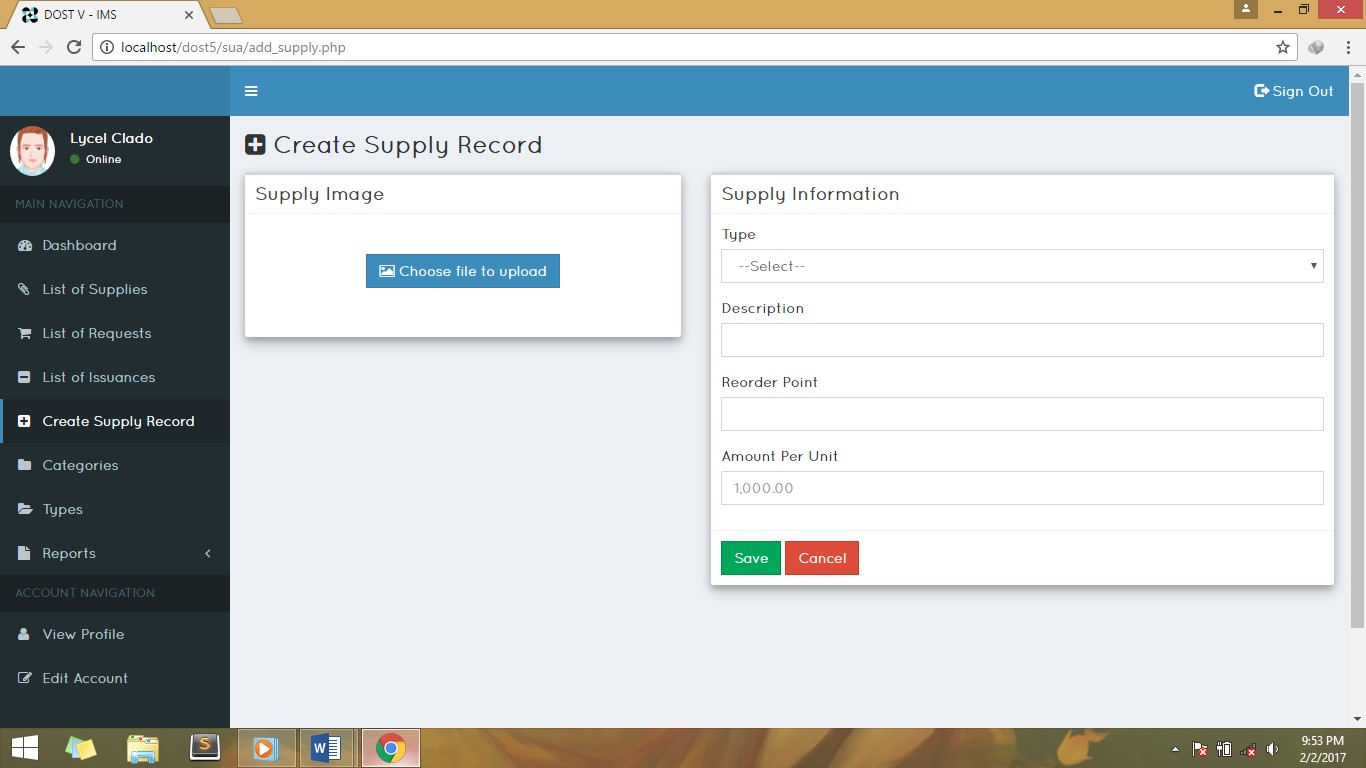
\includegraphics[width=13cm,height=8cm]{image/d3-7.jpg}\\
	Creating Supply Record\\
	\vspace{1.5cm}
	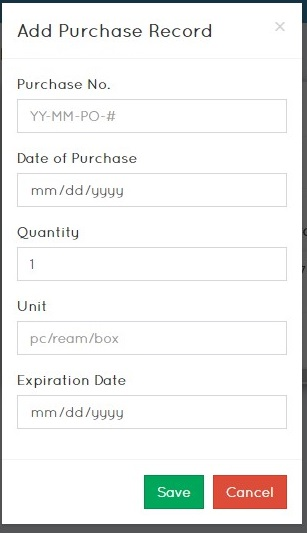
\includegraphics[width=8cm,height=6cm]{image/d3-8.jpg}\\
	Adding Purchase Record\\
	\vspace{1.5cm}
	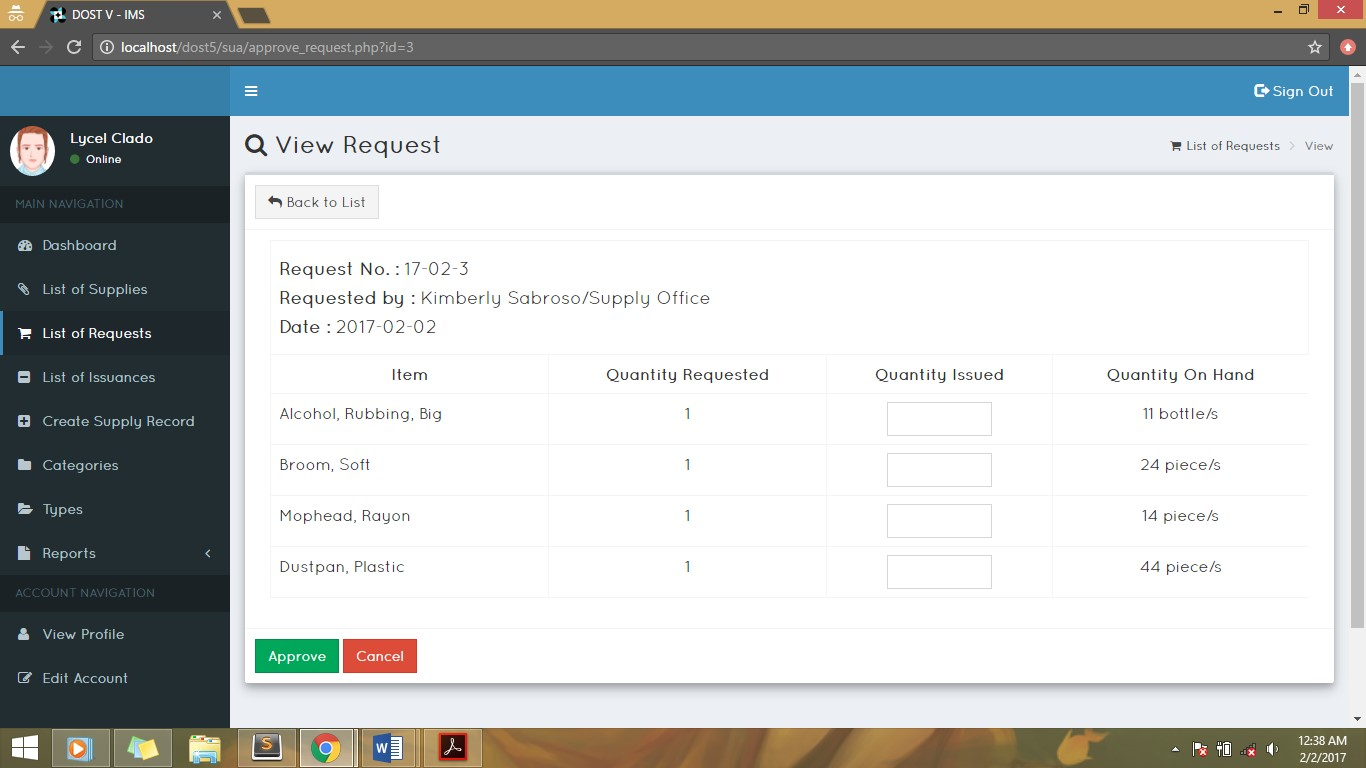
\includegraphics[width=13cm,height=8cm]{image/d3-9.jpg}\\
	Approving Request for Supplies\\
\end{center}


\begin{flushleft}
	\textbf{Equipment Administrator}
\end{flushleft}	

\begin{center}
	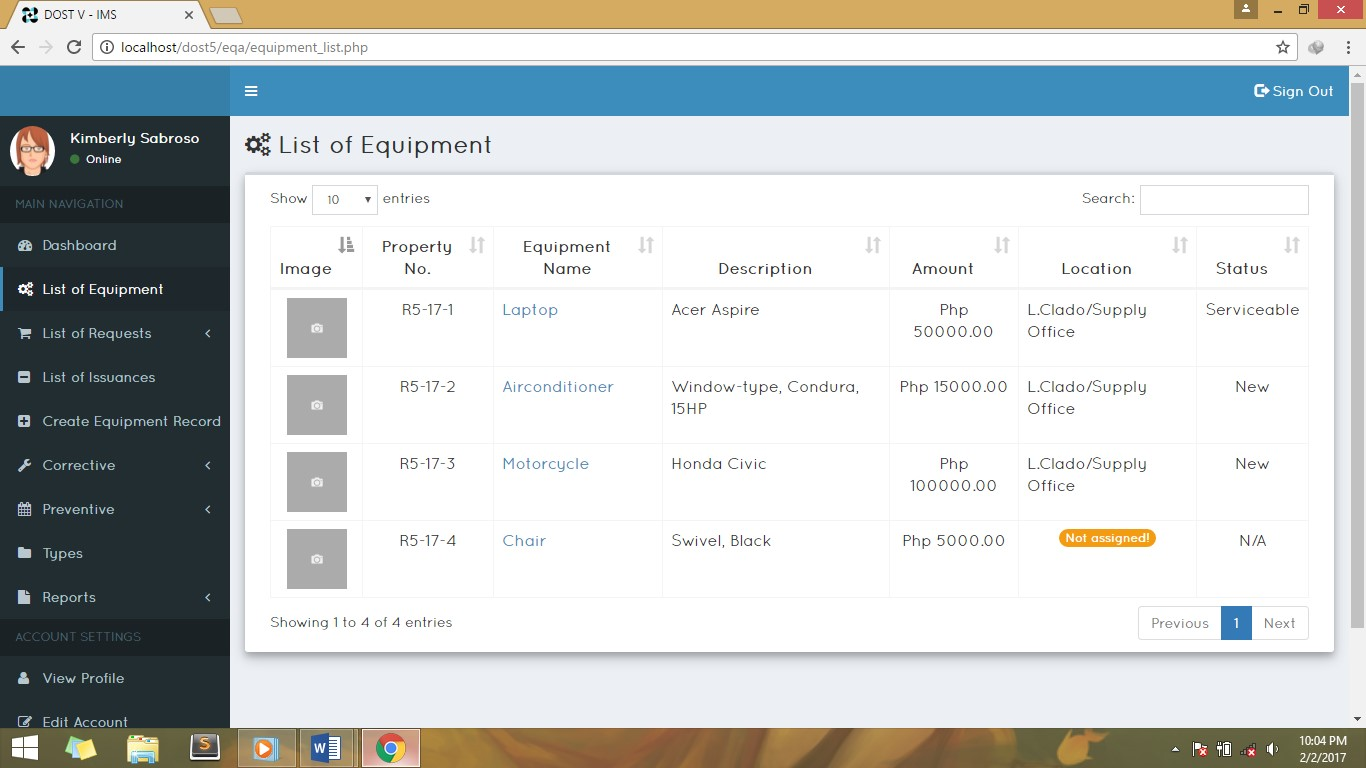
\includegraphics[width=13cm,height=7cm]{image/d3-10.jpg}\\
	List of Equipment \\
	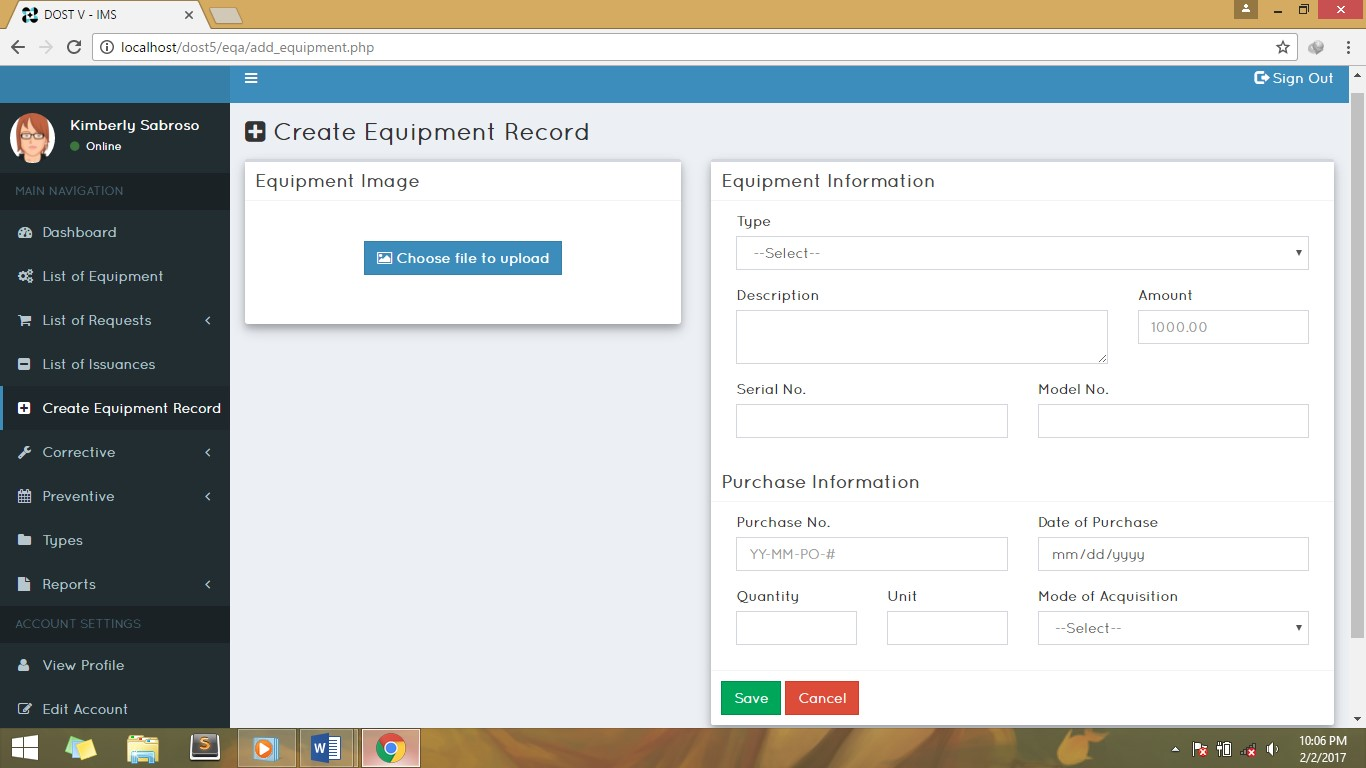
\includegraphics[width=13cm,height=7cm]{image/d3-11.jpg}\\
	Creating Equipment Record\\
	\vspace{1cm}
	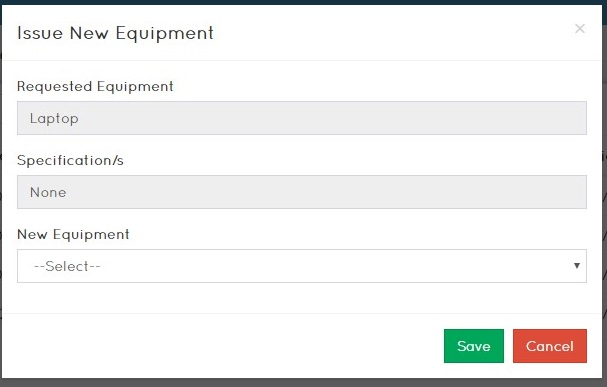
\includegraphics[width=7cm,height=6cm]{image/d3-12.jpg}\\
	Issuing of Equipment\\
	\vspace{1cm}
	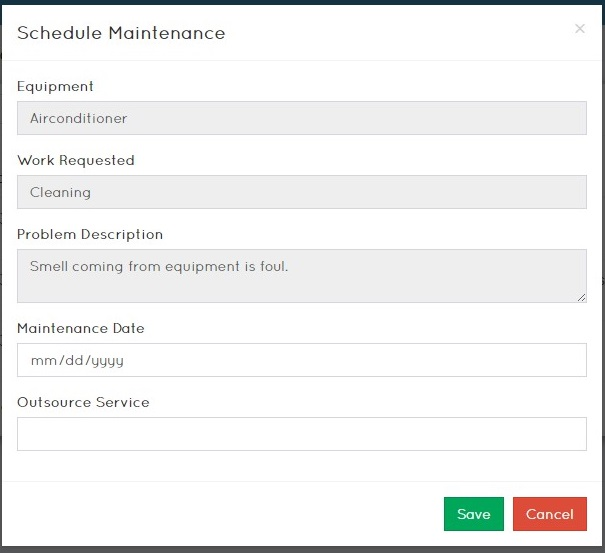
\includegraphics[width=7cm,height=7cm]{image/d3-13.jpg}\\
	Scheduling of Request for Maintenance\\
	\vspace{1cm}
	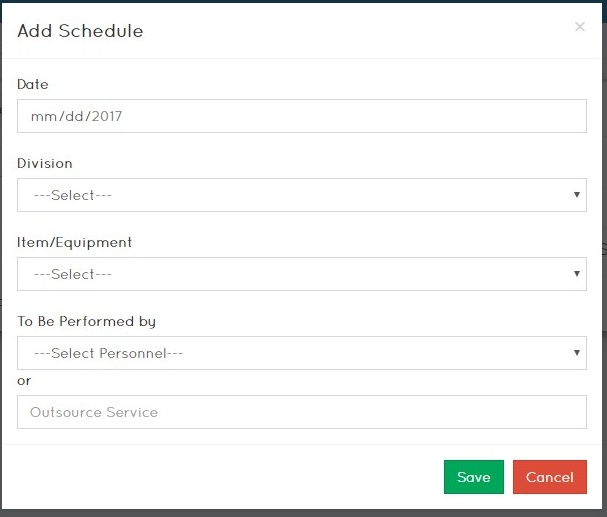
\includegraphics[width=7cm,height=6cm]{image/d3-14.jpg}\\
	Scheduling of Preventive Maintenance\\
	\vspace{1cm}
	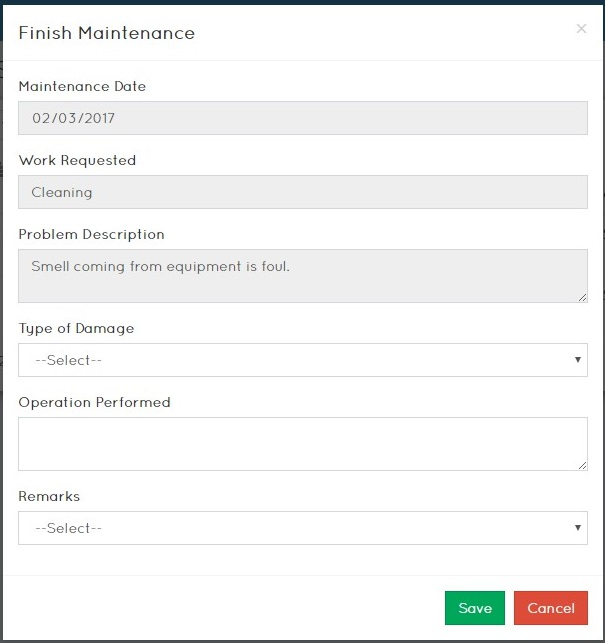
\includegraphics[width=7cm,height=7cm]{image/d3-15.jpg}\\
	Updating Maintenance Record\\
\end{center}

\begin{flushleft}
	\textbf{Super Administrator}
\end{flushleft}	

\begin{center}
	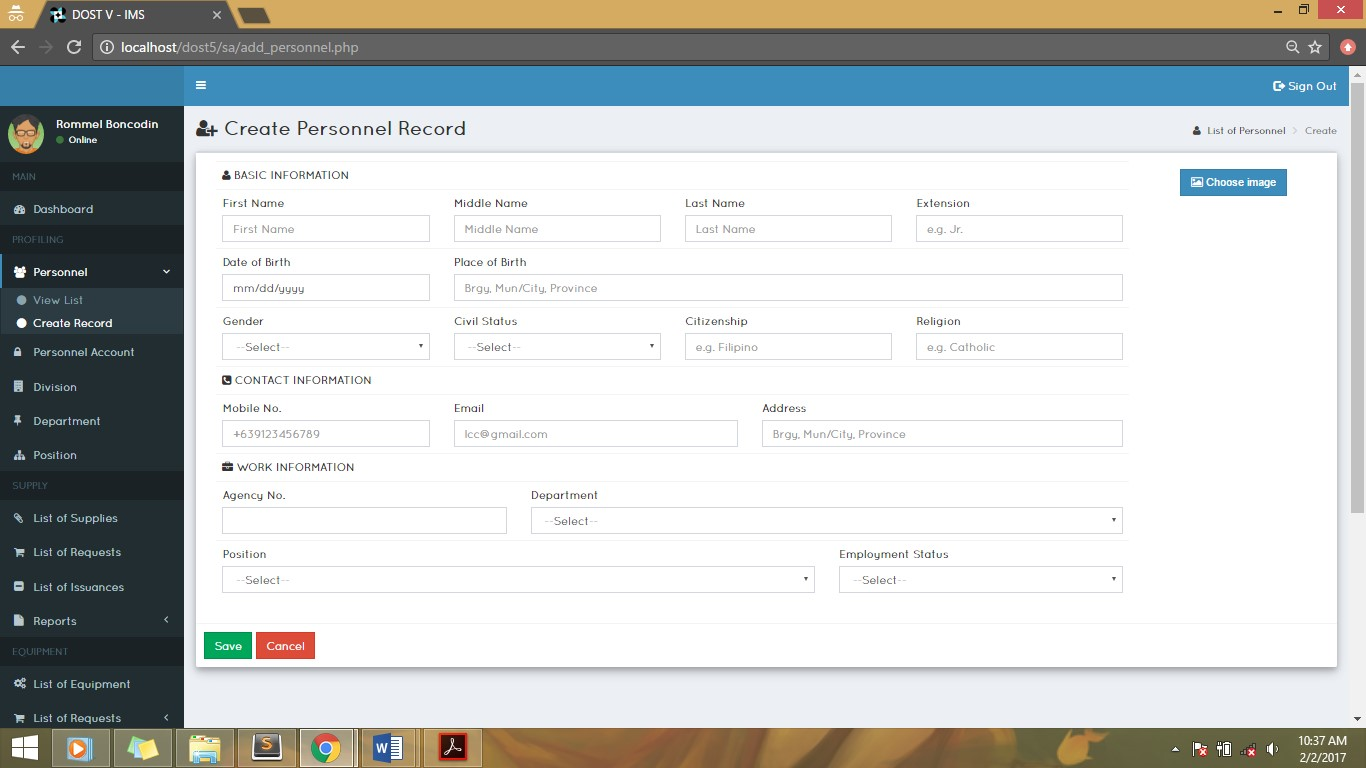
\includegraphics[width=13cm,height=7cm]{image/d3-16.jpg}\\
	Creating Employee Record \\
	\vspace{1cm}
	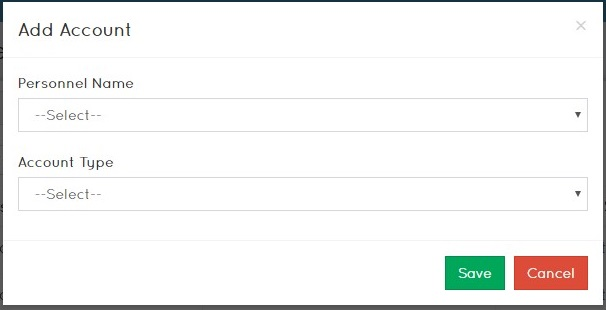
\includegraphics[width=6cm,height=4cm]{image/d3-17.jpg}\\
	Adding Account \\
	\vspace{1cm}
	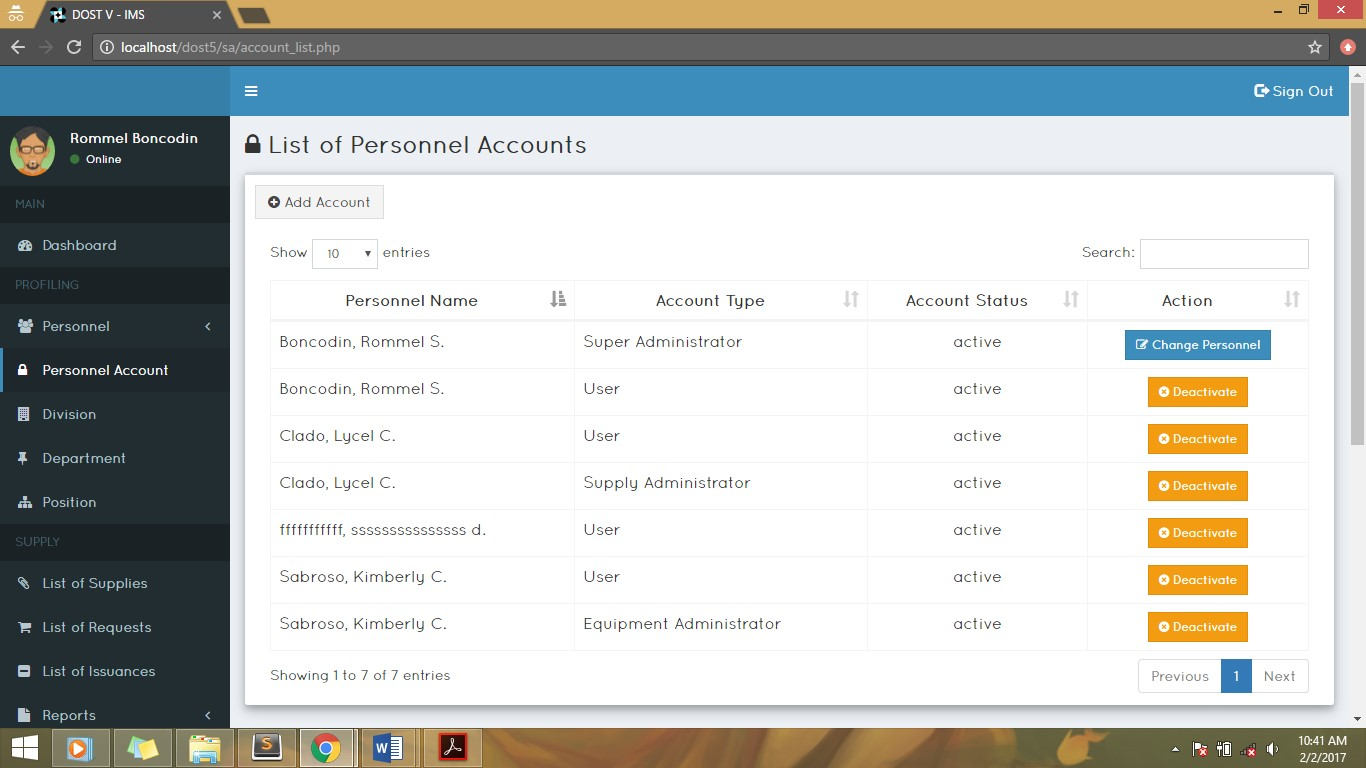
\includegraphics[width=13cm,height=7cm]{image/d3-18.jpg}\\
	Activating/Deactivating Accounts\\
\end{center}
	
	
\end{center}
\vfill

\newpage

\begin{center} 
	\textbf{Deployment Diagram}
\end{center}
\begin{center}
	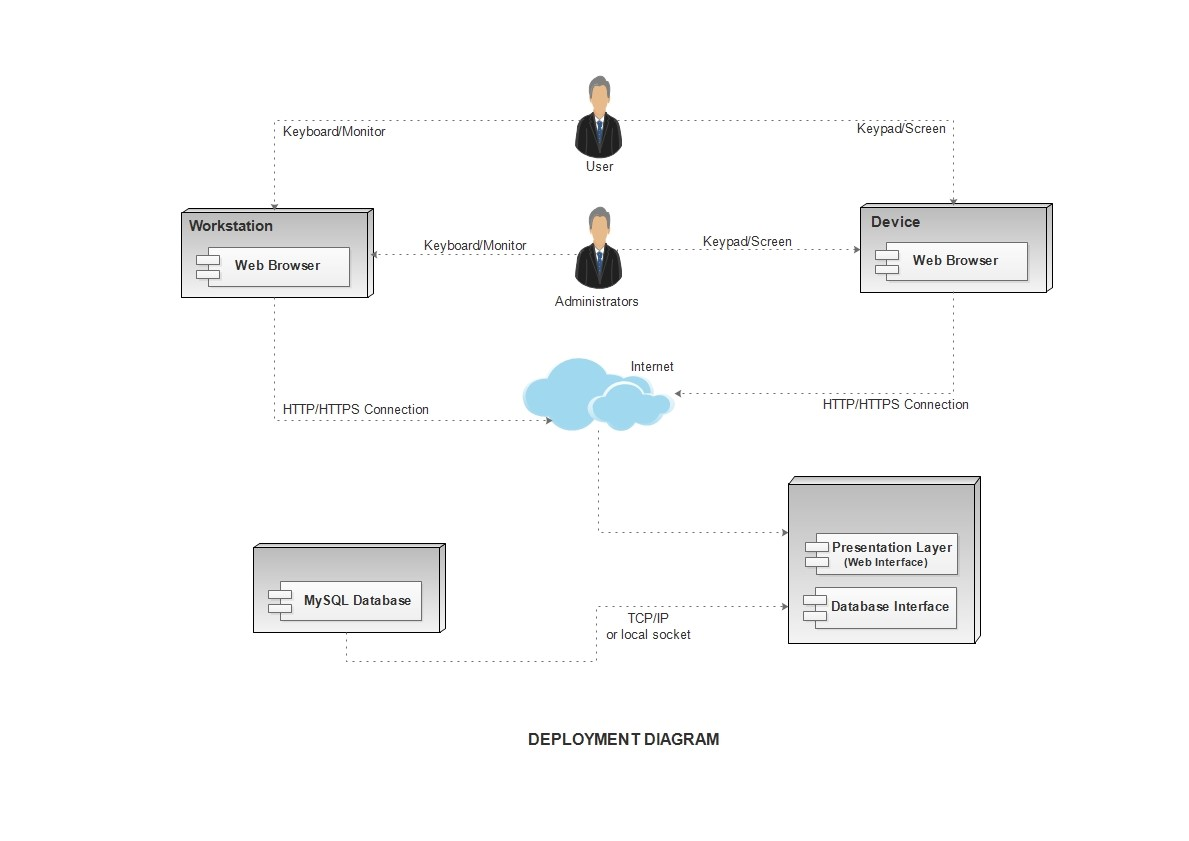
\includegraphics[width=14cm,height=15cm]{image/i.jpg}
\end{center}
\vfill\newpage
\newpage

\begin{center} 
\textbf{\myappendix{Description of Components}}
\end{center}

\begin{center}
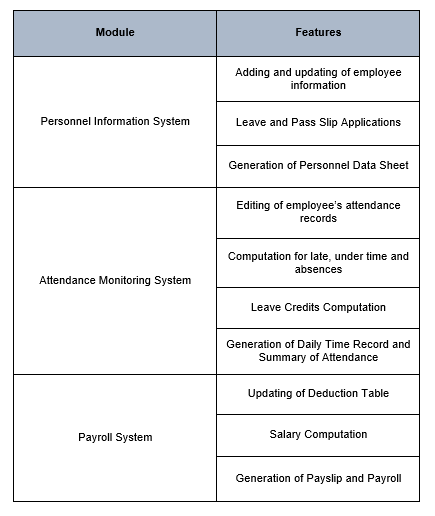
\includegraphics[width=14cm,height=18cm]{image/descriptionofcomponents.PNG}

\end{center}
\newpage
\begin{center} 
	\textbf{\myappendix{Test Cases}}
\end{center}
	
	\begin{center}
	\begin{singlespace}
		\begin{tabular}{ | C{1.5cm} | C{2.5cm} |C{3cm} |C{3cm} |C{3cm} |}  
			\hline
			\textbf{Test Case ID} & \textbf{Test Scenario} & \textbf{Test Steps} & \textbf{Test Data} & \textbf{Actual Results}\\
			\hline 
			TCID001 & Check Login with valid Data & 
			\begin{enumerate}
				\setstretch{1}
				\item [1] Go to link. 
				\item [2] Enter UserID.
				\item [3] Enter password.
				\item [4] Click Submit. 
			\end{enumerate} & Userid = admin1234 Password = passadmin1234 & User was able to Login into application\\
			\hline	
			TCID002 & Check Login with valid Data & 
			\begin{enumerate}
				\setstretch{1}
				\item [1] Go to link. 
				\item [2] Enter UserID.
				\item [3] Enter password.
				\item [4] Click Submit. 
			\end{enumerate} & Userid = admin1234 Password = passadmin1234 & User was able to Login into application\\
			\hline	
		\end{tabular}
	\end{singlespace}
	\end{center}


\newpage
\begin{center} 
	\textbf{\myappendix{Test Documentation}}
\end{center}

\begin{center} 
	\textbf{Pictures During Actual Testing}
\end{center}

\begin{center}
	
\includegraphics[width=9cm,height=6cm]{image/testdoc.jpg}
\end{center}

\begin{center}
	
\includegraphics[width=11cm,height=5.5cm]{image/testdoc2.jpg}
\end{center}

\begin{center}
	
\includegraphics[width=10cm,height=5.5cm]{image/testdoc3.jpg}
\end{center}\newpage
\begin{center} 
	\textbf{\myappendix{User's Manual}}
\end{center}

\noindent
\textbf{Accesing the System}
\begin{enumerate}
	\setstretch{1}
	\item[1.] Install Xampp version 5 or latest
	\item[2.] Run Apache and MySQL
	\item[3.] Go to localhost/new
\end{enumerate}

\noindent
\textbf{Loggin In \\}
\begin{center}
	\includegraphics[width=15cm,height=6cm]{image/login.png}
\end{center}

Ask for your badge number from the Admin, the default password is "password".

\newpage
\noindent
\textbf{ Profile \\}
\begin{center}
	\includegraphics[width=15cm,height=7cm]{image/profile_user.png}
\end{center}

Shown in your profile are 2 panes. The \textbf{left pane} contains all the features or functions you are allowed to do. The \textbf{main pane} contains your personal details, list of all your filed applications and a calendar.

\noindent
\textbf{ 1. Left Pane \\}

\noindent \textbf{User (This option is available to all users) }
\begin{itemize}
	\item Manage and View Payslip – You can view this month’s Payslip or select which month’s Payslip you want to view. \\
	\begin{center}
		\includegraphics[width=15cm,height=7cm]{image/viewPaySlip.png}
	\end{center}
	
	
	\item Summary of Attendance - you can view the summary of your attendance, the total late, undertime and absences for the month. \\
	\begin{center}
		\includegraphics[width=15cm,height=7cm]{image/summaryOfAttendance.png}
	\end{center}
	
\end{itemize}
\newpage
\noindent
\textbf{Personnel Information (Only available for Personnel Information Admins and Superadmin) \\}
\begin{center}
	\includegraphics[width=15cm,height=7cm]{image/PISadmin1.png}
\end{center}

\begin{itemize}
	\item List of Employees
	\begin{enumerate}
		\item[A.] Add an Employee - click the “+” button on the upper right corner. A window will appear where you can enter basic information about the employee \\
		\begin{center}
			\includegraphics[width=8cm,height=8cm]{image/addemp_um.png}
		\end{center}
		
		\item[B.] Show - Click the arrow down button beside the number and choose how many entries you want to view.
		\item[C.] Search - On the textfield type the keyword. It will find the keyword in al the columns.
		\item[D.] Number of Entries and Pages - Shown is the number of entries shown and the total number of entries. The number of pages is also shown, click the page number to view the entries on that page.
	\end{enumerate}
	\item List of Departments
	\begin{enumerate}
		\item[E.]Show - Click the arrow down button beside the number and choose how many entries you want to view.
		\item[F.] Search - On the textfield type the keyword. It will find the keyword in al the columns.
		\item[G.] Number of Entries and Pages - Shown is the number of entries shown and the total number of entries. The number of pages is also shown, click the page number to view the entries on that page.
	\end{enumerate}
\end{itemize}
\begin{center}
	\includegraphics[width=15cm,height=7cm]{image/PISadmin2.png}
\end{center}
\begin{itemize}
	\item List of Positions with Salary Grade 
	\begin{enumerate}
		\item[A.] Add - click the “+” button on the upper right corner. A window will appear where you can enter the position name , the default salary grade is 1. you can edit it later.\\
		\begin{center}
			\includegraphics[width=8cm,height=4cm]{image/addpos_um.png}
		\end{center} 
		\item[B.] Show - Click the arrow down button beside the number and choose how many entries you want to view.
		\item[C.] Search - On the textfield type the keyword. It will find the keyword in al the columns.
		\item[D.] Number of Entries and Pages - Shown is the number of entries shown and the total number of entries. The number of pages is also shown, click the page number to view the entries on that page.
	\end{enumerate}
	\item List of Salary Grade
	\begin{enumerate}
		\item[E.] Add - click the “+” button on the upper right corner. A window will appear where you can enter the amount for the 8 steps\\
		\begin{center}
			\includegraphics[width=8cm,height=7cm]{image/addsalarygrade_um.png}
		\end{center} 
		\item[F.] Show - Click the arrow down button beside the number and choose how many entries you want to view.
		\item[G.] Search - On the textfield type the keyword. It will find the keyword in al the columns.
		\item[H.] Number of Entries and Pages - Shown is the number of entries shown and the total number of entries. The number of pages is also shown, click the page number to view the entries on that page.
	\end{enumerate}
\end{itemize}
\newpage
\noindent
\textbf{Attendance Monitoring (Available to Attendance Monitoring System Admins and Superadmin only)\\ }
\begin{center}
	\includegraphics[width=14cm,height=7cm]{image/ams_um.png}
\end{center} 
\begin{enumerate}
	\item[A.] Manage Holidays -Add or Edit the holidays and Special Events. \\
	\begin{center}
		\includegraphics[width=14cm,height=7cm]{image/Holidays.png}
	\end{center}
	\item[B.] Manage Equivalent Tables – Edit the Equivalent table for Leave Credits. \\
	\begin{center}
		\includegraphics[width=14cm,height=7cm]{image/LCequi.png}
	\end{center}
	\item[C.] Upload DTR – this option is for uploading the CSV file from the Biometrics. \\
	\begin{center}
		\includegraphics[width=8cm,height=4cm]{image/upload.png}
	\end{center}
\end{enumerate}
\newpage
\noindent
\textbf{Payroll (Available to Payroll System Admins and Superadmin only) \\}
\begin{center}
	\includegraphics[width=7cm,height=7cm]{image/PS_um.png}
\end{center} 

\begin{enumerate}
	\item[A.] Manage Deduction Tables – Manage the deduction tables for PAG-IBIG, PhilHealth, Tax and GSIS.
	\begin{center}
		\includegraphics[width=14cm,height=7cm]{image/deducTables.png}
	\end{center} 
	\item[B.] View Payroll -  View the Payroll which contains a list of employees with their gross pay, deductions and net pay.
	\begin{center}
		\includegraphics[width=14cm,height=7cm]{image/Payroll.png}
	\end{center}
\end{enumerate}

\newpage
\noindent
\textbf{ 2. Main Pane \\}
\begin{center}
	\includegraphics[width=15cm,height=7cm]{image/profile_user.png}
\end{center} 

\begin{itemize}
	\item[A.] Recent Activity
	\begin{itemize}
		\item For Users: Contains two tabs: Leave Applications, which shows a list of your filed Leave application; Pass Slips, shows a list of pass slips you filed.
		\item For Attendance Monitoring Admins and Super Admin: Contains two tabs: Leave Applications, which shows a list of all filed Leave applications for approval; Pass Slips, shows a list of pass slips filed for your approval.
	\end{itemize}
	\item Edit Personnel Data Sheet - \\ Enter all your Data, to save the data click the “Submit” button.\\
	\begin{center}
		\includegraphics[width=14cm,height=8cm]{image/editPDS.png}
	\end{center} 
	\item Calendar -
	\begin{center}
		\includegraphics[width=14cm,height=7cm]{image/calendar.png}
	\end{center}
	\begin{itemize}
		\item Check Leave Credits - \\
		To check you leave credits, just click any date on the calendar.\\
		\begin{center}
			\includegraphics[width=13cm,height=8cm]{image/checkLC.png}
		\end{center} 
		\item Apply for Leave - \\
		To apply for Leave, click any date on the calendar and click the “Leave” button. A window will appear where you can enter all your leave details, click the “Submit” button for your application to filed. \\
		\begin{center}
			\includegraphics[width=13cm,height=8cm]{image/Leave.png}
		\end{center}
		\item Apply for Pass Slip - \\
		To apply for Pass Slips, click any date on the calendar and click the “Pass” button. A window will appear where you can enter all your pass slip details, click the “Submit” button for your application to filed. \\
		\begin{center}
			\includegraphics[width=13cm,height=8cm]{image/pass.png}
		\end{center}
		\item View Daily Time Record 
		\begin{center}
			\includegraphics[width=13cm,height=8cm]{image/viewDTR.png}
		\end{center}
	\end{itemize}
\end{itemize}
\newpage
\begin{center}
	\textbf{ \myappendix{Source Codes}}
\end{center}

%\end{center}

\begin{multicols}{2}
	\begin{flushleft}
		\setstretch{1}
		{\fontfamily{qcr}\selectfont
		{\fontsize{9}{10}\selectfont
			
			%\setlength{\columnsep}{3cm}       
			
			\lstinputlisting[caption=\textbf{Getting of Daily Time Record}.]{sourcecodes/getDTR.m}   
			
			\lstinputlisting[caption=\textbf{Getting and Displaying of Leave Application}.]{sourcecodes/getLeave.m}
			
			\lstinputlisting[caption=\textbf{Getting and Displaying of Pass Slip Application}.]{sourcecodes/getPass.m}
			
			\lstinputlisting[caption=\textbf{Checking of changes} if there was any changes made in the system.]{sourcecodes/check_changes.m}
			
			\lstinputlisting[caption=\textbf{Leave Credits} computation.]{sourcecodes/leaveCredits.m}   
			
			\lstinputlisting[caption=\textbf{Add Employee} contains basic information in creating a new account.]{sourcecodes/addEmployee.m}
			
			\lstinputlisting[caption=\textbf{Assign Roles} to an employee to become an admin or from admin to become an employee.]{sourcecodes/assignRoles.m}
			
			\lstinputlisting[caption=\textbf{Getting of employee data for Payroll}.]{sourcecodes/payrollEmpdata.m}
			
		}}
	\end{flushleft}
\end{multicols}\newpage
%\begin{center} 
	\textbf{\myappendix{Certification}}
\end{center}

\begin{center}
	\includegraphics[width=15cm,height=20cm]{image/appendix_k.png}
\end{center}


\newpage
%\begin{center} 
	\textbf{\myappendix{User's Manual}}
\end{center}

\noindent
\textbf{Accesing the System}
\begin{enumerate}
	\setstretch{1}
	\item[1.] Install Xampp version 5 or latest
	\item[2.] Run Apache and MySQL
	\item[3.] Go to localhost/new
\end{enumerate}

\noindent
\textbf{Loggin In \\}
\begin{center}
	\includegraphics[width=15cm,height=6cm]{image/login.png}
\end{center}

Ask for your badge number from the Admin, the default password is "password".

\newpage
\noindent
\textbf{ Profile \\}
\begin{center}
	\includegraphics[width=15cm,height=7cm]{image/profile_user.png}
\end{center}

Shown in your profile are 2 panes. The \textbf{left pane} contains all the features or functions you are allowed to do. The \textbf{main pane} contains your personal details, list of all your filed applications and a calendar.

\noindent
\textbf{ 1. Left Pane \\}

\noindent \textbf{User (This option is available to all users) }
\begin{itemize}
	\item Manage and View Payslip – You can view this month’s Payslip or select which month’s Payslip you want to view. \\
	\begin{center}
		\includegraphics[width=15cm,height=7cm]{image/viewPaySlip.png}
	\end{center}
	
	
	\item Summary of Attendance - you can view the summary of your attendance, the total late, undertime and absences for the month. \\
	\begin{center}
		\includegraphics[width=15cm,height=7cm]{image/summaryOfAttendance.png}
	\end{center}
	
\end{itemize}
\newpage
\noindent
\textbf{Personnel Information (Only available for Personnel Information Admins and Superadmin) \\}
\begin{center}
	\includegraphics[width=15cm,height=7cm]{image/PISadmin1.png}
\end{center}

\begin{itemize}
	\item List of Employees
	\begin{enumerate}
		\item[A.] Add an Employee - click the “+” button on the upper right corner. A window will appear where you can enter basic information about the employee \\
		\begin{center}
			\includegraphics[width=8cm,height=8cm]{image/addemp_um.png}
		\end{center}
		
		\item[B.] Show - Click the arrow down button beside the number and choose how many entries you want to view.
		\item[C.] Search - On the textfield type the keyword. It will find the keyword in al the columns.
		\item[D.] Number of Entries and Pages - Shown is the number of entries shown and the total number of entries. The number of pages is also shown, click the page number to view the entries on that page.
	\end{enumerate}
	\item List of Departments
	\begin{enumerate}
		\item[E.]Show - Click the arrow down button beside the number and choose how many entries you want to view.
		\item[F.] Search - On the textfield type the keyword. It will find the keyword in al the columns.
		\item[G.] Number of Entries and Pages - Shown is the number of entries shown and the total number of entries. The number of pages is also shown, click the page number to view the entries on that page.
	\end{enumerate}
\end{itemize}
\begin{center}
	\includegraphics[width=15cm,height=7cm]{image/PISadmin2.png}
\end{center}
\begin{itemize}
	\item List of Positions with Salary Grade 
	\begin{enumerate}
		\item[A.] Add - click the “+” button on the upper right corner. A window will appear where you can enter the position name , the default salary grade is 1. you can edit it later.\\
		\begin{center}
			\includegraphics[width=8cm,height=4cm]{image/addpos_um.png}
		\end{center} 
		\item[B.] Show - Click the arrow down button beside the number and choose how many entries you want to view.
		\item[C.] Search - On the textfield type the keyword. It will find the keyword in al the columns.
		\item[D.] Number of Entries and Pages - Shown is the number of entries shown and the total number of entries. The number of pages is also shown, click the page number to view the entries on that page.
	\end{enumerate}
	\item List of Salary Grade
	\begin{enumerate}
		\item[E.] Add - click the “+” button on the upper right corner. A window will appear where you can enter the amount for the 8 steps\\
		\begin{center}
			\includegraphics[width=8cm,height=7cm]{image/addsalarygrade_um.png}
		\end{center} 
		\item[F.] Show - Click the arrow down button beside the number and choose how many entries you want to view.
		\item[G.] Search - On the textfield type the keyword. It will find the keyword in al the columns.
		\item[H.] Number of Entries and Pages - Shown is the number of entries shown and the total number of entries. The number of pages is also shown, click the page number to view the entries on that page.
	\end{enumerate}
\end{itemize}
\newpage
\noindent
\textbf{Attendance Monitoring (Available to Attendance Monitoring System Admins and Superadmin only)\\ }
\begin{center}
	\includegraphics[width=14cm,height=7cm]{image/ams_um.png}
\end{center} 
\begin{enumerate}
	\item[A.] Manage Holidays -Add or Edit the holidays and Special Events. \\
	\begin{center}
		\includegraphics[width=14cm,height=7cm]{image/Holidays.png}
	\end{center}
	\item[B.] Manage Equivalent Tables – Edit the Equivalent table for Leave Credits. \\
	\begin{center}
		\includegraphics[width=14cm,height=7cm]{image/LCequi.png}
	\end{center}
	\item[C.] Upload DTR – this option is for uploading the CSV file from the Biometrics. \\
	\begin{center}
		\includegraphics[width=8cm,height=4cm]{image/upload.png}
	\end{center}
\end{enumerate}
\newpage
\noindent
\textbf{Payroll (Available to Payroll System Admins and Superadmin only) \\}
\begin{center}
	\includegraphics[width=7cm,height=7cm]{image/PS_um.png}
\end{center} 

\begin{enumerate}
	\item[A.] Manage Deduction Tables – Manage the deduction tables for PAG-IBIG, PhilHealth, Tax and GSIS.
	\begin{center}
		\includegraphics[width=14cm,height=7cm]{image/deducTables.png}
	\end{center} 
	\item[B.] View Payroll -  View the Payroll which contains a list of employees with their gross pay, deductions and net pay.
	\begin{center}
		\includegraphics[width=14cm,height=7cm]{image/Payroll.png}
	\end{center}
\end{enumerate}

\newpage
\noindent
\textbf{ 2. Main Pane \\}
\begin{center}
	\includegraphics[width=15cm,height=7cm]{image/profile_user.png}
\end{center} 

\begin{itemize}
	\item[A.] Recent Activity
	\begin{itemize}
		\item For Users: Contains two tabs: Leave Applications, which shows a list of your filed Leave application; Pass Slips, shows a list of pass slips you filed.
		\item For Attendance Monitoring Admins and Super Admin: Contains two tabs: Leave Applications, which shows a list of all filed Leave applications for approval; Pass Slips, shows a list of pass slips filed for your approval.
	\end{itemize}
	\item Edit Personnel Data Sheet - \\ Enter all your Data, to save the data click the “Submit” button.\\
	\begin{center}
		\includegraphics[width=14cm,height=8cm]{image/editPDS.png}
	\end{center} 
	\item Calendar -
	\begin{center}
		\includegraphics[width=14cm,height=7cm]{image/calendar.png}
	\end{center}
	\begin{itemize}
		\item Check Leave Credits - \\
		To check you leave credits, just click any date on the calendar.\\
		\begin{center}
			\includegraphics[width=13cm,height=8cm]{image/checkLC.png}
		\end{center} 
		\item Apply for Leave - \\
		To apply for Leave, click any date on the calendar and click the “Leave” button. A window will appear where you can enter all your leave details, click the “Submit” button for your application to filed. \\
		\begin{center}
			\includegraphics[width=13cm,height=8cm]{image/Leave.png}
		\end{center}
		\item Apply for Pass Slip - \\
		To apply for Pass Slips, click any date on the calendar and click the “Pass” button. A window will appear where you can enter all your pass slip details, click the “Submit” button for your application to filed. \\
		\begin{center}
			\includegraphics[width=13cm,height=8cm]{image/pass.png}
		\end{center}
		\item View Daily Time Record 
		\begin{center}
			\includegraphics[width=13cm,height=8cm]{image/viewDTR.png}
		\end{center}
	\end{itemize}
\end{itemize}
\newpage
%\begin{center}
	\textbf{ \myappendix{Source Codes}}
\end{center}

%\end{center}

\begin{multicols}{2}
	\begin{flushleft}
		\setstretch{1}
		{\fontfamily{qcr}\selectfont
		{\fontsize{9}{10}\selectfont
			
			%\setlength{\columnsep}{3cm}       
			
			\lstinputlisting[caption=\textbf{Getting of Daily Time Record}.]{sourcecodes/getDTR.m}   
			
			\lstinputlisting[caption=\textbf{Getting and Displaying of Leave Application}.]{sourcecodes/getLeave.m}
			
			\lstinputlisting[caption=\textbf{Getting and Displaying of Pass Slip Application}.]{sourcecodes/getPass.m}
			
			\lstinputlisting[caption=\textbf{Checking of changes} if there was any changes made in the system.]{sourcecodes/check_changes.m}
			
			\lstinputlisting[caption=\textbf{Leave Credits} computation.]{sourcecodes/leaveCredits.m}   
			
			\lstinputlisting[caption=\textbf{Add Employee} contains basic information in creating a new account.]{sourcecodes/addEmployee.m}
			
			\lstinputlisting[caption=\textbf{Assign Roles} to an employee to become an admin or from admin to become an employee.]{sourcecodes/assignRoles.m}
			
			\lstinputlisting[caption=\textbf{Getting of employee data for Payroll}.]{sourcecodes/payrollEmpdata.m}
			
		}}
	\end{flushleft}
\end{multicols}\newpage
%
%\begin{center} 
    %\textbf{Appendix N}\\


\begin{center}
   \textbf{ \myappendix{Sources Code}}
\end{center}
    
%\end{center}

\begin{multicols}{2}
	\begin{flushleft}
        {\fontfamily{qcr}\selectfont
	
	%\setlength{\columnsep}{5cm}       
	
            \lstinputlisting[caption=\textbf{Getting of Daily Time Record}.]{sourcecodes/getDTR.m}   

            \lstinputlisting[caption=\textbf{Getting and Displaying of Leave Application}.]{sourcecodes/getLeave.m}

            \lstinputlisting[caption=\textbf{Getting and Displaying of Pass Slip Application}.]{sourcecodes/getPass.m}

            \lstinputlisting[caption=\textbf{Checking of changes} if there was any changes made in the system.]{sourcecodes/check_changes.m}

            \lstinputlisting[caption=\textbf{Leave Credits} computation.]{sourcecodes/leaveCredits.m}   

            \lstinputlisting[caption=\textbf{Add Employee} contains basic information in creating a new account.]{sourcecodes/addEmployee.m}

            \lstinputlisting[caption=\textbf{Assign Roles} to an employee to become an admin or from admin to become an employee.]{sourcecodes/assignRoles.m}

            \lstinputlisting[caption=\textbf{Getting of employee data for Payroll}.]{sourcecodes/payrollEmpdata.m}

            %\lstinputlisting[caption=\textbf{Borrow Books page} the information of borrower and the book to be borrow property-no and date borrow.]{sourcecodes/add_borrower.m}

            %\lstinputlisting[caption=\textbf{Add Book page} contains all the information needed.]{sourcecodes/add_book.m}

            %\lstinputlisting[caption=\textbf{Inventory of Library   Holdings page} list of all books article cd journal magazine newspaper and thesis) with additional features that count the no. of times borrowed.]{sourcecodes/inventory.m}

            %\lstinputlisting[caption=\textbf{Monitor the most borrowed books total of all library holdings newly acquired books.} All the information are attach with printable reports.]{sourcecodes/monitor.m}

            %\lstinputlisting[caption=\textbf{Search for library holdings information}  where they can view the information add copy edit information print book card or details and delete information.]{sourcecodes/list_textbook.m}

            %\lstinputlisting[caption=\textbf{Catalogue} books by author subject and title also they can print the catalog card of the books.]{sourcecodes/catalogue_author.m}

            %\lstinputlisting[caption=\textbf{Indexing} of library holdings to easily track the library holdings by simply clicking the letter. And pop out  all the valid information.]{sourcecodes/indexing.m}

        }
\end{flushleft}
 \end{multicols}



 \newpage


\clearpage
    \vspace*{\fill}
        \begin{center}
            \begin{minipage}{.6\textwidth}
                
\section {CURRICULUM VITAE}
                
            \end{minipage}
        \end{center}
    \vfill
\clearpage

\newpage

\centering{\textbf{CURRICULUM VITAE}}
\begin{flushright}
	\raisebox{-5,1cm}[1][0cm]
	{\includegraphics[width=5.5cm]{image/pic.png}}
\end{flushright}


\begin{itemize}
	\vspace{-25mm}
	\item []\textbf{ PERSONAL INFORMATION}
	\begin{itemize}
		\setstretch{1}
		\item  \textbf{Name:} {Zenica B. Torre}
		\item  \textbf{Age:} {18}
		\item  \textbf{Gender:} {Female}
		\item  \textbf{Birth Date}: {December 6, 1998}
		\item  \textbf{Address:} {Brgy. 13 Bacacay, Albay}
		\item  \textbf{Civil Status:} {Single}
		\item  \textbf{Citizenship:} {Filipino}
		\item  \textbf{Religion:} {Roman Catholic}
		\item  \textbf{Parents:} {}
		\item  \textbf{Email:} {torrezenica@gmail.com}
	\end{itemize}
	\item []\textbf{EDUCATIONAL BACKGROUND}
	\begin{itemize}
		\setstretch{1}
		\item \textbf{Tertiary Education}
		\begin{itemize}
			\item School: Bicol University College of Science
			\item Address: Rizal St. Legazpi City, Albay
			\item Academic Program: Bachelor of Science in Information Technology
			\item Duration: 2012-2016
		\end{itemize}
		\item \textbf{Secondary Education}
		\begin{itemize}
			\item School: Bicol University High School Department
			\item Address: Rizal St. Legazpi City, Albay
			\item Duration: 2008-2012
		\end{itemize}
		\item \textbf{Elementary Education}
		\begin{itemize}
			\item School: Bicol University Integrated Laboratory School
			\item Address: Rizal St. Legazpi City, Albay
			\item Duration: 2002-2008
		\end{itemize}
	\end{itemize}
\end{itemize}
	
\newpage

\centering{\textbf{CURRICULUM VITAE}}
\begin{flushright}
	\raisebox{-5,1cm}[1][0cm]
	{\includegraphics[width=5.5cm]{image/pic.png}}
\end{flushright}


\begin{itemize}
	\vspace{-25mm}
	\item []\textbf{ PERSONAL INFORMATION}
	\begin{itemize}
		\setstretch{1}
		\item  \textbf{Name:} {Jhona Jane B. Francisco}
		\item  \textbf{Age:} {18}
		\item  \textbf{Gender:} {Female}
		\item  \textbf{Birth Date}: {December 6, 1998}
		\item  \textbf{Address:} {Brgy. 13 Bacacay, Albay}
		\item  \textbf{Civil Status:} {Single}
		\item  \textbf{Citizenship:} {Filipino}
		\item  \textbf{Religion:} {Roman Catholic}
		\item  \textbf{Parents:} {}
		\item  \textbf{Email:} {torrezenica@gmail.com}
	\end{itemize}
	\item []\textbf{EDUCATIONAL BACKGROUND}
	\begin{itemize}
		\setstretch{1}
		\item \textbf{Tertiary Education}
		\begin{itemize}
			\item School: Bicol University College of Science
			\item Address: Rizal St. Legazpi City, Albay
			\item Academic Program: Bachelor of Science in Information Technology
			\item Duration: 2012-2016
		\end{itemize}
		\item \textbf{Secondary Education}
		\begin{itemize}
			\item School: Bicol University High School Department
			\item Address: Rizal St. Legazpi City, Albay
			\item Duration: 2008-2012
		\end{itemize}
		\item \textbf{Elementary Education}
		\begin{itemize}
			\item School: Bicol University Integrated Laboratory School
			\item Address: Rizal St. Legazpi City, Albay
			\item Duration: 2002-2008
		\end{itemize}
	\end{itemize}
\end{itemize}

\newpage

\centering{\textbf{CURRICULUM VITAE}}
\begin{flushright}
	\raisebox{-5,1cm}[1][0cm]
	{\includegraphics[width=5.5cm]{image/pic.png}}
\end{flushright}


\begin{itemize}
	\vspace{-25mm}
	\item []\textbf{ PERSONAL INFORMATION}
	\begin{itemize}
		\setstretch{1}
		\item  \textbf{Name:} {Kianne Marie T. Paguntalan}
		\item  \textbf{Age:} {18}
		\item  \textbf{Gender:} {Female}
		\item  \textbf{Birth Date}: {December 6, 1998}
		\item  \textbf{Address:} {Brgy. 13 Bacacay, Albay}
		\item  \textbf{Civil Status:} {Single}
		\item  \textbf{Citizenship:} {Filipino}
		\item  \textbf{Religion:} {Roman Catholic}
		\item  \textbf{Parents:} {}
		\item  \textbf{Email:} {torrezenica@gmail.com}
	\end{itemize}
	\item []\textbf{EDUCATIONAL BACKGROUND}
	\begin{itemize}
		\setstretch{1}
		\item \textbf{Tertiary Education}
		\begin{itemize}
			\item School: Bicol University College of Science
			\item Address: Rizal St. Legazpi City, Albay
			\item Academic Program: Bachelor of Science in Information Technology
			\item Duration: 2012-2016
		\end{itemize}
		\item \textbf{Secondary Education}
		\begin{itemize}
			\item School: Bicol University High School Department
			\item Address: Rizal St. Legazpi City, Albay
			\item Duration: 2008-2012
		\end{itemize}
		\item \textbf{Elementary Education}
		\begin{itemize}
			\item School: Bicol University Integrated Laboratory School
			\item Address: Rizal St. Legazpi City, Albay
			\item Duration: 2002-2008
		\end{itemize}
	\end{itemize}
\end{itemize}	
	
	
	







\end{document}
